%% TODO Recheck Author guidelines: https://dl.acm.org/journal/pacmpl/author-guidelines

\documentclass[acmsmall,%
  screen,%
  % review,%% TODO make sure review is turned on before submitting, it turns line numbers on
  % anonymous,%% TODO make sure anonymous is set before submitting and that there are no mentions of our names.
  nonacm%
]{acmart}

%% Warning: Command \showhyphens has changed.
%% Once overleaf updates to TexLive 2026, it will be fixed
%% https://github.com/borisveytsman/acmart/issues/577

%% Warning: Class acmart Warning: \vspace should only be used to provide space above/below surrounding objects on input line 894.
%% Seems vspace is being called by includegraphics
%% https://github.com/borisveytsman/acmart/issues/552
% \let\oldvspace\vspace
% \renewcommand{\vspace}[1]{%
%   \typeout{VSPACE CALLED: #1}%
%   \tracingmacros=1
%   \oldvspace{#1}%
%   \tracingmacros=0
% }

%% \BibTeX command to typeset BibTeX logo in the docs
\AtBeginDocument{%
  \providecommand\BibTeX{{%
    Bib\TeX}}}

%% TODO: Get copyright when completing the rights form
%% Rights management information.  This information is sent to you
%% when you complete the rights form.  These commands have SAMPLE
%% values in them; it is your responsibility as an author to replace
%% the commands and values with those provided to you when you
%% complete the rights form.
\setcopyright{acmlicensed}
\copyrightyear{2018}
\acmYear{2018}
\acmDOI{XXXXXXX.XXXXXXX}

%% TODO: Get Submission ID
%% Submission ID.
%% Use this when submitting an article to a sponsored event. You'll
%% receive a unique submission ID from the organizers
%% of the event, and this ID should be used as the parameter to this command.
%%\acmSubmissionID{123-A56-BU3}

%% TODO:
%% Look at the sample-*-biblatex.tex files for templates showcasing
%% the biblatex styles.

% the mandatory bibstyle
\bibliographystyle{ACM-Reference-Format}
\citestyle{acmauthoryear}

%%%%% BEGIN: Author additions to style %%%%%%

%% Begin Lean code style
% Lean code: Correctly display unicode characters in lstlisting
% We copied this from a previously acccepted ITP article: https://arxiv.org/abs/2309.07252
\usepackage{listings} % package listings is in the list of accepted packages https://authors.acm.org/proceedings/production-information/accepted-latex-packages
% 
\usepackage{color} % package color is in the allowed list of accepted packages https://authors.acm.org/proceedings/production-information/accepted-latex-packages
\definecolor{keywordcolor}{rgb}{0.7, 0.1, 0.1}   % red
\definecolor{tacticcolor}{rgb}{0.0, 0.1, 0.6}    % blue
\definecolor{commentcolor}{rgb}{0.4, 0.4, 0.4}   % grey
\definecolor{symbolcolor}{rgb}{0.0, 0.1, 0.6}    % blue
\definecolor{sortcolor}{rgb}{0.1, 0.5, 0.1}      % green
\definecolor{stringcolor}{rgb}{0.1, 0.5, 0.1}    % green
\definecolor{attributecolor}{rgb}{0.7, 0.1, 0.1} % red
\def\lstlanguagefiles{lstlean.tex}
% set default language
\lstset{language=lean,
backgroundcolor=,
extendedchars=true,
stringstyle=\color{stringcolor},
escapeinside={/*!}{!*/}, % https://tex.stackexchange.com/questions/413891/hyperlink-text-inside-lstlisting
}
%% End Lean code style

%% Begin other additions

%% Reference code via a hyperref
\usepackage{xspace} % package xspace is in the allowed list of accepted packages https://authors.acm.org/proceedings/production-information/accepted-latex-packages
\newcommand{\link}[2]{\mbox{\hyperref[#2]{\lstinline{#1}}}\xspace}
\newcommand{\jsonlink}[2]{\mbox{\hyperref[#2]{\lstinline[language=json]{#1}}}\xspace}
\newcommand{\refcode}[1]{\hyperref[#1]{\lstinline[breaklines=true,literate={\_}{}{0\discretionary{\_}{}{\_}}]{#1}}\xspace}

%% Names
\newcommand{\Hedge}{\refcode{Hedge}}
\newcommand{\Node}{\link{Hedge.Node}{Hedge}}
\newcommand{\GrammarKatydidDerive}{\link{Grammar.Katydid.derive}{def Grammar.Katydid.derive}}
\newcommand{\RegexCharDerive}{\link{Regex.Char.derive}{def Regex.Char.derive}}
\newcommand{\Grammar}{\link{Grammar}{Grammar}}
\newcommand{\Regex}{\link{Regex}{Regex}}
\newcommand{\Rule}{\link{Regex (φ × Ref n)}{Grammar}}
\newcommand{\Reference}{\link{Ref n}{Ref}}
\newcommand{\RegexKatydidDerive}{\link{Regex.Katydid.derive}{def Regex.Katydid.derive}}
\newcommand{\symcount}{\link{symcount}{def symcount}}
\newcommand{\enter}{\link{enter}{def enter}}
\newcommand{\leave}{\link{leave}{def leave}}
\newcommand{\extract}{\link{extract}{def extract}}
\newcommand{\replace}{\link{replace}{def replace}}
\newcommand{\RegexDerive}{\link{Regex.derive}{def Regex.derive}}
\newcommand{\JSONmembersRuleDerive}{\link{Grammar.JSONmembers.derive}{def Grammar.JSONmembers.derive}}
\newcommand{\RegexPointDerive}{\link{Regex.Point.derive}{def Regex.Point.derive}}
\newcommand{\decideRel}{\link{decideRel}{def decideRel}}
\newcommand{\RuleDenote}{\link{Rule.denote}{def Rule.denote}}
\newcommand{\RegexDenote}{\link{Regex.denote}{def Regex.denote}}
\newcommand{\LangDerive}{\link{Lang.derive}{def Lang.derive}}
\newcommand{\Lang}{\link{Lang}{def Lang}}
\newcommand{\TheoremDeriveCommutes}{\refcode{theorem derive_commutes}}
\newcommand{\RegexValidate}{\link{Regex.validate}{def Regex.validate}}
\newcommand{\HedgeNodeLabel}{\link{Hedge.Node.label}{Hedge}}
\newcommand{\RegexNull}{\link{Regex.null}{def Regex.null}}
\newcommand{\LangNull}{\link{Lang.null}{def Lang.null}}
\newcommand{\GrammarMemoizeFilter}{\link{Grammar.Memoize.filter}{def Grammar.Memoize.filter}}
\newcommand{\MemoizeKatydid}{\link{MemoizeKatydid}{MemoizeKatydid}}
\newcommand{\AnyEqPred}{\link{Pred}{AnyEqPred}}
\newcommand{\Token}{\link{Token}{Token}}

%% Lean Logo
\newcommand{\Lean}{%
  Lean\xspace%
}

%% BEGIN: Define JSON syntax highlighting
\definecolor{delim}{RGB}{20,105,176}
\definecolor{numb}{RGB}{106, 109, 32}
\definecolor{string}{rgb}{0.64,0.08,0.08}
\lstdefinelanguage{json}{
    showspaces=false,
    showtabs=false,
    breaklines=true,
    postbreak=\raisebox{0ex}[0ex][0ex]{\ensuremath{\color{gray}\hookrightarrow\space}},
    breakatwhitespace=true,
    basicstyle=\ttfamily\small,
    upquote=true,
    morestring=[b]",
    stringstyle=\color{string},
    literate=
     *{0}{{{\color{numb}0}}}{1}
      {1}{{{\color{numb}1}}}{1}
      {2}{{{\color{numb}2}}}{1}
      {3}{{{\color{numb}3}}}{1}
      {4}{{{\color{numb}4}}}{1}
      {5}{{{\color{numb}5}}}{1}
      {6}{{{\color{numb}6}}}{1}
      {7}{{{\color{numb}7}}}{1}
      {8}{{{\color{numb}8}}}{1}
      {9}{{{\color{numb}9}}}{1}
      {\{}{{{\color{delim}{\{}}}}{1}
      {\}}{{{\color{delim}{\}}}}}{1}
      {[}{{{\color{delim}{[}}}}{1}
      {]}{{{\color{delim}{]}}}}{1},
}
%% END: Define JSON syntax highlighting

%% Used to stop bad hyphenations.
\hyphenation{name/JSON}

%% Used for Cref to create capatilized references to Section and Fig.
\usepackage[nameinlink]{cleveref}

%% Only used for checkmark and cross in table
\usepackage{pifont}\newcommand{\cmark}{\ding{51}}\newcommand{\xmark}{\ding{55}}

%%%%% END: Author aditions to style %%%%%%

\begin{document}

\title{Memoized Derivatives for Fast Filtering and Schema Validation of Semi-Structured Data}

\author{Walter {Schulze}}
\email{mail@awalterschulze.org}
\orcid{0009-0002-4400-1606}
\affiliation{%
  \institution{Stellenbosch University}
  \city{Stellenbosch}
  \country{South Africa}}

\author{Brink {van der Merwe}}
\email{abvdm@sun.ac.za}
\orcid{0000-0001-5010-9934}
\affiliation{%
  \institution{Stellenbosch University}
  \city{Stellenbosch}
  \country{South Africa}}

\author{Paul {Cadman}}
\email{research@paulcadman.dev}
\orcid{0009-0002-5034-3514}
\affiliation{%
  \institution{Independent Researcher}
  \city{London}
  \country{United Kingdom}}

%% TODO Add Christiaan
\author{Christiaan {Maasdorp}}
\email{chm2@sun.ac.za}
\orcid{0000-0002-9248-4756}
\affiliation{%
  \institution{Stellenbosch University}
  \city{Stellenbosch}
  \country{South Africa}}

%%
%% By default, the full list of authors will be used in the page
%% headers. Often, this list is too long, and will overlap
%% other information printed in the page headers. This command allows
%% the author to define a more concise list
%% of authors' names for this purpose.
\renewcommand{\shortauthors}{Schulze et al.}

%%
%% The code below is generated by the tool at http://dl.acm.org/ccs.cfm.
\begin{CCSXML}
<ccs2012>
   <concept>
       <concept_id>10011007.10011006.10011039.10011311</concept_id>
       <concept_desc>Software and its engineering~Semantics</concept_desc>
       <concept_significance>500</concept_significance>
       </concept>
   <concept>
       <concept_id>10011007.10010940.10010992.10010998.10010999</concept_id>
       <concept_desc>Software and its engineering~Software verification</concept_desc>
       <concept_significance>500</concept_significance>
       </concept>
   <concept>
       <concept_id>10003752.10003766.10003776</concept_id>
       <concept_desc>Theory of computation~Regular languages</concept_desc>
       <concept_significance>500</concept_significance>
       </concept>
   <concept>
       <concept_id>10010405.10010497.10010498</concept_id>
       <concept_desc>Applied computing~Document searching</concept_desc>
       <concept_significance>500</concept_significance>
       </concept>
 </ccs2012>
\end{CCSXML}

\ccsdesc[500]{Software and its engineering~Semantics}
\ccsdesc[500]{Software and its engineering~Software verification}
\ccsdesc[500]{Theory of computation~Regular languages}
\ccsdesc[500]{Applied computing~Document searching}
%% End of generated code

%%
%% Keywords. The author(s) should pick words that accurately describe
%% the work being presented. Separate the keywords with commas.
\keywords{regular hedge grammar, high-performance filtering, schema validation, formal verification, Brzozowski derivative, Lean, RelaxNG, JSONSchema, Protocol Buffers.} 

\received{1 July 2026}
% \received[revised]{12 March 2009}
% \received[accepted]{5 June 2009}

\begin{abstract}
We present a high-performance filtering and schema-validation algorithm based on Brzozowski’s derivatives extended to regular hedge grammars for semi-structured data.
Our algorithm inherits the expressiveness of regular hedge grammars to support a wide range of schema languages and serialization formats, such as JSONSchema, XML/RelaxNG and Protocol Buffers.
High performance is achieved by refactoring the derivative algorithm to make it more amenable to memoization of hedges and elimination of heap allocations.
We verify the correctness of our memoization technique for regular hedge grammars in Lean.
This is the first proof of correctness in an interactive theorem prover of a derivative algorithm for regular hedge grammars or any schema language.
We benchmark an implementation of our memoization technique in Golang, against several other JSONSchema implementations, showing it can filter millions of records per second.
\end{abstract}

%%
%% This command processes the author and affiliation and title
%% information and builds the first part of the formatted document.
\maketitle

\section{Introduction}

We present a verified filtering algorithm for semi-structured data formats such as XML, JSON and Protocol Buffers~\cite{protobuf}, designed for high-throughput use cases involving millions of records per second.
The memoization technique is formally verified in Lean~\cite{lean4}.

Our approach is based on Brzozowski derivatives~\cite{brzozowski1964derivatives}, a classical technique for recognizing regular languages.
We adapt this derivative algorithm to operate on regular hedge grammars, which generalize regular expressions to \emph{hedges}, or informally, to tree-shaped data. 
These grammars form the foundation of schema languages such as RelaxNG~\cite{hosoya2010foundations} and JSONSchema~\cite{jsonschemafoundations}.
They enable expressive constraints over ordered and unordered element sequences, nesting, repetition and recursion.
We start with a simple JSONSchema example to illustrate and motivate our approach.

\subsection{JSONSchema Example}

To illustrate the application of Brzozowski's derivative algorithm to JSONSchema, we consider a simplified version of a blog post schema~\cite{jsonschemaexamples}:
\begin{lstlisting}[language=json,label=jsonschema_blogpost]
{ "title": "small jsonschema for a blogpost",
  "type":"object", "additionalProperties":false, "required": ["content", "author"],
  "properties": {
    "content": { "type":"string" },
    "author": { "$ref":"#/definitions/user-profile" } },
  "definitions": { "user-profile": {
    "type": "object", "additionalProperties":false, "required": ["username"], 
    "properties": {
      "username": { "type":"string" },
      "email": { "type":"string", "format":"email" } } } } }
\end{lstlisting}
The schema requires a content field and an author object, the latter of which comprises a username and an optional email address; for example: \lstinline[language=json]|{"content": "Dragons", "author": {"username": "Khaleesi"}}|

Brzozowski’s derivative algorithm for regular expressions takes a regular expression and a sequence of characters as input.
To facilitate the derivation, we utilize the ``JSONmembers'' algorithm—a term we adopt for the procedure introduced by~\citet{holstege2019application}—which flattens the JSON object into a sequence of key-value pairs: \lstinline[language=json]|[{"content": "Dragons"}, {"author": {"username": "Khaleesi"}}]|.
Subsequently, the algorithm computes the derivative of the schema with respect to the first member.
This operation yields a residual schema, analogous to how the derivative of a regular expression represents the remaining language after a single character is matched.
The algorithm proceeds recursively, computing the derivative for each subsequent member of the input. Finally, we determine if the resulting schema accepts the empty object, analogous to checking whether a derived regular expression is nullable (i.e., matches the empty string).
Computing the derivative of the schema with respect to the first member, \lstinline[language=json]|{"content": "Dragons"}|, yields:
\begin{lstlisting}[language=json]
{ "type": "object", "additionalProperties": false, "required": ["author"], 
  "properties": { "author": { "$ref":"#/definitions/user-profile" } } ... }
\end{lstlisting}
We see that we have matched the content property and only the author property is still required.

We wish to use memoization to improve the performance, as is done for regular expressions.
In the case of regular expressions, the input alphabet of characters is small and has low variance and results in lots of successful lookups (hits) in the memoization table.
Unfortunately the input alphabet of JSON values is large and unbounded, which is demonstrated in the example above, each blog post will have different content, which will result in zero hits in the memoization table.
We refactor the derivative function into a composition of three steps: \enter, evaluate predicates and \leave.
In the case of JSONSchema, the first step (the \enter function) extracts a list of properties that we need to match, this includes the field name or predicate and accompanying child schema.
The second step checks whether the input field name matches the field name or predicate collected by \enter and recurses down, until a list of booleans is returned that indicates whether each field name and child schema sucessfully matched.
Finally, the \leave function re-integrates the results (list of booleans) back into the schema and computes the derivative.
The \enter and \leave functions are memoized, since they only depend on the schema and a list of booleans and do not depend on the input alphabet.
Given the resulting schema where we still need to match the author and the input that is left to validate is \lstinline[language=json]|[{"author": {"username": "Khaleesi"}}]|, we can complete the validation using our new Katydid\footnote{A Katydid is a leaf insect that camouflages (requires filtering) itself in trees (data structures)} algorithm.
We can start by applying \enter to extract the properties \lstinline[language=json]|[{"author": { "$ref": "#/definitions/user-profile" }}]|.
In second step we check which properties matches the \lstinline[language=json]|"author"| field name and lookup any references, which gives us the following singleton list:
\begin{lstlisting}[language=json]
[{ "type": "object", "additionalProperties": false, "required": ["username"],
   "properties": { "username": {"type":"string"},
                   "email": {"type":"string", "format":"email"}}}]
\end{lstlisting}
We recurse down and apply the \enter function again, giving us the following two properties:
\begin{lstlisting}[language=json]
[{"username": {"type": "string"}}, {"email": {"type":"string", "format":"email"}}]
\end{lstlisting}
We apply second step, evaluate the predicates, using with the \lstinline[language=json]|"username"| field name and get the following schemas to evaluate on the children:
\begin{lstlisting}[language=json]
[{"type": "string"}, {"not": {}}]
\end{lstlisting}
We matched the \lstinline[language=json]|"username"| field, but not the \lstinline[language=json]|"email"| field, so we pass down the second element as the schema that matches nothing \lstinline[language=json]|{"not": {}}|.
We are at the bottom of the JSON input, so we evaluate the string \lstinline[language=json]|"Khaleesi"| against the predicates, which results in the list \lstinline[language=json]|[true, false]|.
Now we can apply the final step, the \leave function, reintegrate the results and take the derivative.
We apply the derivative, with the knowledge that the username property matched and the email property did not:
\begin{lstlisting}[language=json]
[{ "type": "object", "additionalProperties": false, "required": [],
   "properties": { "email": {"type":"string", "format":"email"}}}]
\end{lstlisting}
We have no more input, and we recurse back up, but we first need to check whether this schema matched the input, by checking whether the resulting schema matches the empty object.
We check the nullability of each schema in the list, which results in \lstinline[language=json]|[true]|, since the schema has no more required fields and the email was optional.
Again we can apply the \leave function given the parent schema and the nullability results:
\begin{lstlisting}[language=json]
{ "type": "object", "additionalProperties": false, "required": [], 
  "properties": {}, "definitions": { ... } }
\end{lstlisting}
We check whether the final schema matches the empty object, which it does, which means the input is valid given this schema.
Note: there are technical details we brushed over for the purpose of creating an intuition of the algorithm, that we will clear up in future sections.

\subsection{Motivation and Contributions}

%% Rewrote this in the following paragraph:
% Currently, there are two algorithms (excluding the one introduced in this paper) that process hedges using derivatives, one for RelaxNG~\cite{relaxng2001simple} and another applied to JSONSchema~\cite{holstege2019application}.
% Both of these algorithms have shortcomings in what can be memoized which we resolve with our new Katydid algorithm\footnote{A Katydid is a leaf insect that camouflages (requires filtering) itself in trees (data structures)}. 
We have discussed two algorithms that process schemas using derivatives: the JSONmembers algorithm and our new Katydid algorithm, which is the focus of this paper.
The final derivative algorithm for schemas that exists is for an XML schema language RelaxNG~\cite{relaxng2001simple} and is the original inspiration for this work.
It converts the schema into a Balanced Context Free Grammar (BCFG), on the fly, as it applies derivatives.
It implements efficient memoization, that only uses the shema and element names in the memoization table.
The element names have a large alphabet, but low variance, so it results in lots of hits of the memoization table.
The big improvement our algorithm makes over RelaxNG is that our algorithm can optionally create a fully memoized table before seeing any input and this table will take up finite space, because our memoization technique is bounded, since we model a schema as a regular hedge grammar and not a BCFG.

The motivation for this work arose in the context of a proprietary distributed database that stored denormalized Protocol Buffers, where schema-based filtering needed to be performed at scale.
To meet production-level performance requirements we implemented the memoization technique in Golang~\cite{golang} with a strong emphasis on avoiding heap allocations.
The benchmarks of this implementation demonstrate its ability to filter data at high speeds and that it competes with other JSONSchema validators.
We verify the correctness by proving, in Lean, that the implementation of the JSONmembers~\citet{holstege2019application} algorithm and Katydid's memoization algorithm faithfully matches the semantics of a regular hedge grammar.

\subsection{Outline}

The remainder of the paper is structured as follows. 
\Cref{section_algorithm} continues the explanation of the Katydid algorithm. \Cref{section_verification} presents formal verifications. 
In \Cref{section_go}, we describe the Go implementation and in \Cref{section_benchmarks}, we provide benchmark results against other JSONSchema implementations.
\Cref{section_related} covers related work and \Cref{section_future} outlines the directions for future research.

Definitions and proofs are presented in the syntax of the Lean theorem prover~\cite{lean4} and are available in the supplementary material~\footnote{No part of the Lean code (including the formal proofs) or the Golang code was created with the aid of GenAI (LLMs).}.
Lean tutorials are available online~\cite{learnlean}. 

\section{The Katydid Algorithm}\label{section_algorithm}

In this section, we describe the Katydid algorithm, a \emph{resource-effective} memoized filtering algorithm, defined as \GrammarMemoizeFilter.
We define its building blocks \enter, \leave, \RegexKatydidDerive and \GrammarKatydidDerive, but we start by defining \emph{regular expressions}, which is the core of \emph{regular hedge grammars}, our generic schema language.

\subsection{Regular Expressions}

A \emph{regular expression} is defined as~\cite{brzozowski1964derivatives, elliott2021symbolic}:
\begin{lstlisting}[label=Regex]
inductive Regex (σ: Type) where
  | emptyset | emptystr | symbol (s: σ) | or (r1 r2: Regex σ)
  | concat (r1 r2: Regex σ) | star (r1: Regex σ) | interleave (r1 r2: Regex σ)
\end{lstlisting}
We include the \lstinline{interleave} operator to handle semi-structured data, for example, unordered JSON members and XML attributes~\cite{hosoya2010foundations}.
We also support the \lstinline{and} and \lstinline{complement} operators in our definitions and proofs in the supplementary material, but omit them here for brevity.
We define additional operators as helper functions:
\begin{lstlisting}
def onlyif (cond: Prop) [dcond: Decidable cond] (r: Regex σ): Regex σ :=
  if cond then r else emptyset
def oneOrMore (r: Regex σ) := concat r (star r)
def optional (r: Regex σ) := or r emptystr
def starAny: Regex σ := complement emptyset
def contains (r: Regex σ) := concat starAny (concat r starAny)
\end{lstlisting}
These extra operators and helper functions are used by both RelaxNG and JSONSchema, as well as in our examples and benchmarks.

\subsection{Derivative of a Regular Expression}

Filtering through a list of strings (which are represented as a \lstinline{List (List α)}) requires validating these strings against a regular expression. This is achieved by successively taking derivatives with respect to each symbol in a string, and at the end, checking whether the resulting expression matches the empty string~\cite{brzozowski1964derivatives, reexamined}:
\begin{lstlisting}[label=def Regex.validate]
def Regex.validate (Φ: σ → α → Bool) (r: Regex σ) (xs: List α): Bool :=
  null (List.foldl (derive Φ) r xs)
def Regex.filter (Φ: σ → α → Bool) (r: Regex σ) (xs: List (List α)) :=
  List.filter (validate Φ r) xs
\end{lstlisting}
The derivative of a regular expression yields the expression that remains to be matched after consuming a list element~\cite{brzozowski1964derivatives, elliott2021symbolic, reexamined}:
\begin{lstlisting}[label=def Regex.derive]
def Regex.derive (Φ: σ → α → Bool) (r: Regex σ) (a: α): Regex σ := match r with
  | emptyset => emptyset | emptystr => emptyset
  | symbol s => onlyif (Φ s a) emptystr
  | or r1 r2 => or (derive Φ r1 a) (derive Φ r2 a)
  | concat r1 r2 => or
      (concat (derive Φ r1 a) r2)
      (onlyif (null r1) (derive Φ r2 a))
  | star r1 => concat (derive Φ r1 a) (star r1)
  | interleave r1 r2 => or
      (interleave (derive Φ r1 a) r2)
      (interleave (derive Φ r2 a) r1)
\end{lstlisting}
The \lstinline{null} function returns whether a regular expression matches the empty string~\cite{brzozowski1964derivatives, elliott2021symbolic, reexamined}:
\begin{lstlisting}[label=def Regex.null]
def Regex.null: (r: Regex σ) → Bool
  | emptyset => false | emptystr => true | symbol _ => false
  | or r1 r2 => (null r1 || null r2) | concat r1 r2 => (null r1 && null r2)
  | star _ => true | interleave r1 r2 => (null r1 && null r2)
\end{lstlisting}
We define \RegexPointDerive, a variation of the original \RegexDerive function designed for more efficient memoization. 
By removing the dependency on specific list elements, it serves as a streamlined building block for the subsequent \leave function, to reintegrate results and take the derivative:
\begin{lstlisting}[label=def Regex.Point.derive]
def Regex.Point.derive: (r: Regex (σ × Bool)) → Regex σ
  | emptyset => emptyset | emptystr => emptyset
  | symbol (_, res) => onlyif res emptystr
  | or r1 r2 => or (derive r1) (derive r2)
  | concat r1 r2 => or
      (concat (derive r1) (first r2))
      (onlyif (null r1) (derive r2))
  | star r1 => concat (derive r1) (star (first r1))
  | interleave r1 r2 => or
      (interleave (derive r1) (first r2))
      (interleave (derive r2) (first r1))
\end{lstlisting}
Instead of the original symbols, each position now contains a tuple comprising the symbol and its predicate evaluation result.
This pair can be interpreted as a point on the graph of the predicate function.
In the \lstinline{symbol} case, the result is checked, but in all other cases the original derivative algorithm is applied by either calling derive or retrieving the original regular expression with the \lstinline{first} function, which maps over the regular expression as a Functor:
\begin{lstlisting}
def Regex.Point.first (r: Regex (α × β)): Regex α := Regex.map r (fun (s,_) => s)
\end{lstlisting}
We can prove that these two derivative functions are equivalent:
\begin{lstlisting}[label=theorem regex_derive_is_point_derive]
theorem regex_derive_is_point_derive (Φ: σ → α → Bool) (r: Regex σ) (a: α):
  Regex.derive Φ r a = Regex.Point.derive (r.map (fun s => (s, Φ s a)))
\end{lstlisting}
The proof follows from induction on \lstinline{r}.

With the foundations of regular expressions in place, we now return to regular hedge grammars.

\subsection{Regular Hedge Grammars}

\emph{Regular hedge grammars} constitute the theoretical framework most applicable to XML~\cite{hosoya2010foundations} and other serialization formats.
Any XML, JSON or Protocol Buffers data can be viewed as a \Hedge and schema languages, such as RelaxNG, DTD~\cite{dtd}, XMLSchema~\cite{xmlschema} and JSONSchema~\cite{jsonschemafoundations} can all be translated to \emph{regular hedge grammars}~\cite{murata2005taxonomy} barring the JSONSchema \lstinline{uniqueItems} operator, which is not regular~\cite{holstege2019application}.

A \emph{hedge} is an ordered list of unranked trees~\cite{tata} used to model semi-structured data formats. In Lean, we define a \Hedge inductively as follows:
\begin{lstlisting}[label=Hedge]
inductive Hedge.Node (α: Type) where
  | node (label: α) (children: List (Hedge.Node α))
abbrev Hedge α := List (Hedge.Node α)
\end{lstlisting}

We borrow our definition of \emph{regular hedge grammars} from \cite{murata2005taxonomy}, which in turn extends the definition of regular tree grammars from \cite{tata}.
\begin{definition}
\label{definition_grammar}
A \emph{regular hedge grammar} is a tuple $(N, T, Start, Prods)$ where:
\begin{itemize}
    \item $N$ is a finite set of non-terminals;
    \item $T$ is a finite set of terminals;
    \item $Start$ is a regular expression over $T \times N$;
    \item $Prods$ is a set of production rules of the form $X \rightarrow r$, where $X \in N$ and $r$ is a regular expression over $T \times N$.
\end{itemize}
\end{definition}

A \emph{symbolic regular hedge grammar} is a generalization of a regular hedge grammar that is paired with a decidable predicate (\lstinline{Φ: φ → α → Bool}), where $T$ is a finite set of symbolic predicates (\lstinline{φ}) over a possibly infinite alphabet (\lstinline{α}).
We represent symbolic regular hedge grammars in Lean as follows:
\begin{lstlisting}[label=Grammar]
structure Grammar (n: Nat) (φ: Type) where
  start: Regex (φ × Ref n)
  prods: Vector (Regex (φ × Ref n)) n
\end{lstlisting}
In the rest of this section we justify the representation.

Non-terminals are represented as a reference \Reference, which is the abbreviation of the set of natural numbers smaller than \lstinline{n}:
\begin{lstlisting}[label=Ref]
abbrev Ref (n: Nat) := Fin n
def lookup (G: Grammar n φ) (ref: Ref n): Regex (φ × Ref n) :=
  Vector.get G.prods ref
\end{lstlisting}
The start and production rules are represented as a \Rule, which is the product of the predicate \lstinline{φ} and the reference.
The indices of the \lstinline{Vector} of production rules are used for the non-terminals, which allows us to write a \lstinline{lookup} function that always returns a unique rule.
Our definition does not allow multiple rules per non-terminal, but this can easily be accommodated using the \lstinline{Regex.or} operator.

These grammars also have useful theoretical properties.
They are closed under union, intersection and complement. 
Their decidable properties include: satisfiability and checking whether one grammar is a subset of another, which is used for type checking~\cite{hosoya2003xduce}.
Each recursion from a lookup only occurs after an evaluation of a predicate \lstinline{φ}.
This disallows arbitrary context-free grammars (CFGs) with undecidable properties~\cite{hosoya2003xduce}.

The following is an example of a simple inductive predicate type, \lstinline{Pred}, together with its corresponding decidable evaluation function \lstinline{Pred.evalb}:
\begin{lstlisting}[label=AnyEqPred]
inductive Pred (α: Type) where | any | eq (t: α)
def Pred.evalb {α: Type} [DecidableEq α] (p: Pred α) (x: α): Bool := match p with
  | Pred.eq y => x = y
  | Pred.any => true
\end{lstlisting}
In practice the predicate type includes complex nested functions such as Unicode normalization, case folding and validating JSONSchema formats, such as email, ipv4, date, etc.

The following example illustrates a regular hedge grammar:
\begin{lstlisting}[label=def example_grammar_doc]
def example_grammar_doc: Grammar 3 (Pred String) :=
  Grammar.mk (start := Regex.symbol (Pred.eq "doc", 0))
    (prods := #v[
      Regex.oneOrMore (Regex.symbol (Pred.eq "p", 1)),
      Regex.symbol (Pred.any, 2),
      Regex.emptystr,
    ])
\end{lstlisting}
It validates the XML snippet \lstinline{<doc><p><pcdata/></p><p><br/></p></doc>}.
We now proceed to describe the \RegexKatydidDerive function, the key to \GrammarKatydidDerive.

%% Moved here from the introduction
\subsection{Our Memoization Solution}

We wish to use memoization to improve the performance of derivative-based filtering over regular hedge grammars.
To characterize when memoization helps in this setting, we make the following definitions:
A function is \emph{memoizable} if its input parameters can be hashed and have decidable equality. 
We express this in Lean using a Monad \lstinline{m} for stateful caching:
\begin{lstlisting}[label=Memoize]
class Memoize [DecidableEq α] [Hashable α] {β: α -> Type} (f: (a: α) → β a)
  (m: Type -> Type u) where call: (a: α) -> m { b: β a // b = f a }
\end{lstlisting}
Other formalizations~\cite{formalmem} additionally have an invariant that input and output values have to be stored, but the \lstinline{Memoize} class allows various caching strategies, including limited space strategies.
Memoization of a function is \emph{resource-effective} when its lookup hit rate grows with the number of calls to that function. 
This occurs when the variance of the input parameters is small, so repeated calls to the function reuse memoized results.
The problem addressed by this paper is to find an algorithm for the derivative of a regular hedge grammar that is memoizable in a resource-effective way.

Let us first review memoization for the ordinary regular expression derivative~\cite{brzozowski1964derivatives}:
\begin{lstlisting}[label=def Regex.Char.derive]
def Regex.Char.derive (r: Regex Char) (a: Char): Regex Char
\end{lstlisting}
Memoization of this function is resource-effective, because the variance of the input parameters is small and the number of different regular expressions is bounded by smart constructors that simplify regular expressions on construction~\cite{reexamined}.
String validation can be performed by lazily constructing a deterministic finite automaton (DFA) using memoization: the initial regular expression acts as the start state, transitions are given by the derivative function, and every distinct regular expression produced by the derivative function becomes a new state. 
As more strings are processed, the lazily constructed fragment of the DFA incrementally expands, allowing it to filter subsequent strings more efficiently~\cite{reexamined}.

To define the derivative of a regular hedge grammar, we need a more general version of the regular expression derivative function that is capable of supporting a \Node input alphabet. 
We achieve this by using a symbolic derivative~\cite{stanford2021symbolic} over a generic input alphabet (\lstinline{α}), a decidable predicate (\lstinline{Φ: σ → α → Bool}) and a separate generic parameter for the regular expression (\lstinline{σ}):
\begin{lstlisting}
def Regex.derive (Φ: σ → α → Bool) (r: Regex σ) (a: α): Regex σ
theorem gen_derive: Regex.Char.derive r a = Regex.derive (fun s a => s == a) r a
\end{lstlisting}
In \RegexCharDerive, the symbol \lstinline{σ} is of the same type as the alphabet \lstinline{α}, but in the general case, the symbol can represent an inductive predicate type, as given in the example \AnyEqPred earlier, where \lstinline{Φ} is the evaluation function \link{Pred.evalb}{AnyEqPred}.

The uncurried symbolic \RegexDerive function is memoizable for a given \lstinline{Φ} and the memoization is resource-effective if the variance on the input parameters is small.
When using \RegexDerive for regular hedge grammars the input alphabet is of type \Node. 
In this case, the memoization of \RegexDerive is not resource-effective, because elements of \Node are trees that can have unbounded depth.

Of the current algorithms, JSONmembers explicitly notes that it does not have resource-effective memoization~\cite{holstege2019application}, while the RelaxNG~\cite{relaxng2001simple} algorithm decomposes the derivative function into smaller components that can be memoized, exploiting the limited variation in XML element nodes.
However, this memoization strategy is not fully resource-effective, because the text nodes have a large and highly variable string alphabet.
To address the challenge of this high variability, they only memoize element nodes and not text nodes.
Also, the memoization technique is unbounded in the number of entries to be memoized.
The table grows on inputs with new element names or deeper recursion.

We restructure the symbolic derivative function to make it more amenable to resource-effective memoization.
The refactored function, \RegexKatydidDerive, is a composition of three functions, two of which are resource-effective to memoize.
First, the \enter function extracts the relevant symbols from the regular expression.
Next, we map the predicate \lstinline{Φ} over the symbols.
Finally, the \leave function re-integrates the results back into the regular expression and computes the derivative.

The two functions (\enter and \leave) are resource-effective for memoization, since they do not depend on the input alphabet:
\begin{lstlisting}[label=def Regex.Katydid.derive]
def enter (r: Regex σ): Vector σ (symcount r)
def leave (r: Regex σ) (bools: Vector Bool (symcount r)): Regex σ
def Regex.Katydid.derive (Φ: σ → Bool) (r: Regex σ): Regex σ :=
  enter r |> Vector.map Φ |> leave r
\end{lstlisting}
Note that \symcount returns the number of symbols in a regular expression and the predicate \lstinline{Φ: σ → Bool} is similar to the predicate in \RegexDerive with the alphabet (\lstinline{α}) partially applied.
We name the functions \enter and \leave to reflect that they correspond to entering and leaving a \Node.
The predicate must be defined to handle the recursive nature of the regular hedge grammar and \Node in a way that utilizes these memoized functions.

\subsection{Enter and Leave}
\label{section_enter_and_leave}

The \GrammarKatydidDerive function is defined using \RegexKatydidDerive, which is defined using the two memoizable functions \enter and \leave.
The \enter function is memoized over the \Regex parameter, whereas \leave is memoized over the product of the \Regex and the evaluated symbols, \lstinline{Vector Bool (symcount r)}.
The \symcount function determines the number of symbols in a regular expression:
\begin{lstlisting}[label=def symcount]
def symcount (r: Regex σ): Nat
#guard symcount (or (symbol 'a') (star (symbol 'b'))) = 2
\end{lstlisting}

The \enter function returns a \lstinline{Vector} of the symbols contained in the regular expression:
\begin{lstlisting}[label=def enter]
def enter (r: Regex σ): Vector σ (symcount r) := (extract r).2
#guard enter (or (symbol 'a') (star (symbol 'b'))) = #v['a','b']
\end{lstlisting}

The symbols are extracted from the regular expression, using the \extract function.
The \extract function returns a \lstinline{Vector} of symbols and a regular expression, where all the symbols have been replaced with indexes into the \lstinline{Vector} from where their original symbols can be retrieved:
\begin{lstlisting}[label=def extract]
def extract (r: Regex σ): Regex (Fin (symcount r)) × Vector σ (symcount r)
#guard extract (or (symbol 'a') (star (symbol 'b')))
  = ((or (symbol 0) (star (symbol 1))), #v['a', 'b'])
\end{lstlisting}

The next step is to evaluate all the symbols by applying \lstinline{Vector.map Φ}.
If care is not taken, this would trigger a heap allocation in Golang, which is costly in the context of this algorithm.
There are several ways to avoid this heap allocation.
In Golang, one can pre-allocate a reusable buffer.
In Lean, we define an alternative to the memoized \enter function, \lstinline{IfExpr.enter}, which returns a nested if expression over the symbols and all possible boolean \lstinline{Vector} combinations.
The definitions and proofs are available in the supplementary material.
The drawback of \lstinline{IfExpr.enter} is an exponential blow-up in the space required for memoization.

The \leave function zips the evaluated results with the original input symbols and replaces these back into the \Regex to create a \lstinline{Regex (σ × Bool)}.
Finally, \leave applies the derivative using \RegexPointDerive:
\begin{lstlisting}[label=def leave]
def leave (r: Regex σ) (bools: Vector Bool (symcount r)): Regex σ :=
  let points: Vector (σ × Bool) (symcount r) := Vector.zip (extract r).2 bools
  let rpoint: Regex (σ × Bool) := replace (extract r).1 points
  Regex.Point.derive rpoint
\end{lstlisting}

The \replace function takes the regular expression with indexes and a \lstinline{Vector} of symbols to be reinserted into the \Regex:
\begin{lstlisting}[label=def replace]
def replace (r: Regex (Fin n)) (xs: Vector σ n): Regex σ
#guard replace (or (symbol 0) (star (symbol 1))) #v['a', 'b']
  = (or (symbol 'a') (star (symbol 'b')))
\end{lstlisting}
This implies that the \extract and \replace functions form an isomorphism. 
\begin{lstlisting}[label=theorem extract_replace_is_id]
theorem extract_replace_is_id (r: Regex σ):
  r = replace (extract r).1 (extract r).2
\end{lstlisting}
More importantly, this allows us to extract all symbols, apply a function to them, and then reinsert them, which is equivalent to mapping over the \Regex as a Functor, using \lstinline{Regex.map}:
\begin{lstlisting}[label=theorem extract_replace_is_map]
theorem extract_replace_is_map (r: Regex α) (f: α → β):
  Regex.map r f = replace (extract r).1 (Vector.map f (extract r).2)
\end{lstlisting}
Unfolding \enter and \leave yields exactly this behaviour:
\begin{lstlisting}
theorem derive_unfolds_to_map (Φ: σ → α → Bool) (r: Regex σ) (a: α):
  Regex.Katydid.derive (flip Φ a) r = Regex.Point.derive
    (replace (extract r).1 (Vector.map (fun s => (s, Φ s a)) (extract r).2))
\end{lstlisting}
In this case, the mapped function \lstinline{f} is \lstinline{fun x => (x, Φ x a)}.
With the \RegexKatydidDerive algorithm defined, let us move on to its role in regular hedge grammars.

\subsection{Derivative of a Regular Hedge Grammar}

The derivative of a regular hedge grammar can be defined analogously to that of a regular expression, with special handling required for the \lstinline{symbol} case:

\begin{lstlisting}[label=def Grammar.JSONmembers.derive]
def Grammar.JSONmembers.derive (G: Grammar n φ) (Φ: φ → α → Bool)
  (r: Regex (φ × Ref n)) (node: Node α): Regex (φ × Ref n) := match r with
  | Regex.symbol (pred, ref) => let ⟨label, children⟩ := node
    Regex.onlyif (Φ pred label
      /\ Regex.null (List.foldl (derive G Φ) (G.lookup ref) children)
    ) Regex.emptystr
  ...
  termination_by (node, r)
\end{lstlisting}
This approach mirrors a derivative algorithm previously applied to JSONSchema~\cite{holstege2019application}, which we refer to as the JSONmembers algorithm for simplicity.

Unfortunately, this approach is not resource-effective to memoize, which motivates the introduction of the Katydid algorithm; again, it requires special handling of the \lstinline{symbol} case, but does so within the \lstinline{nodePred} predicate.
We also implement and verify a memoized variant of this algorithm that supports filtering; however, we first present the non-memoized version, as it forms the foundation of our memoized algorithm:
\begin{lstlisting}[label=def Grammar.Katydid.derive]
def Grammar.Katydid.derive (G: Grammar n φ) (Φ: φ → α → Bool)
  (r: Regex (φ × Ref n)) (node: Node α): Regex (φ × Ref n) :=
  let nodePred := fun ((labelPred, ref): (φ × Ref n)) =>
    let ⟨label, children⟩ := node
    let childr := if Φ labelPred label then G.lookup ref else Regex.emptyset
    Regex.null (List.foldl (Grammar.Katydid.derive G Φ) childr children)
  Regex.Katydid.derive nodePred r -- enter r |> Vector.map nodePred |> leave r
\end{lstlisting}
In both cases, if \lstinline{labelPred} matches the \lstinline{label}, we compute the derivative of the referenced regular expression and fold it over the children of the \Node.
Notice that this folding is the same as the folding done when validating a string, see \RegexValidate.
Since regular expressions and labels are both predicates, their conjunction provides a natural mechanism for recursive \Hedge validation.
Also observe that \RegexKatydidDerive takes a partially applied predicate, where the \lstinline{α} has already been applied.
This is done to make termination obvious to the checker, since \GrammarKatydidDerive is the function that destructs the \Node.

Both derivative functions can be used either to validate a hedge against a regular hedge grammar or to filter a list of hedges:
\begin{lstlisting}
def validate (G: Grammar n φ) (Φ: φ → α → Bool) (nodes: Hedge α): Bool :=
  Regex.null (List.foldl (derive G Φ) G.start nodes)
def filter (G: Grammar n φ) (Φ: φ → α → Bool) (hedges: List (Hedge α)) := 
  List.filter (validate G Φ) hedges
\end{lstlisting}

\subsection{Adding Memoization}

We define memoize versions of the derivative, validate and filter functions, for both regular expressions and regular hedge grammars.
Here is a filter type signature as an example:
\begin{lstlisting}[label=def Grammar.Memoize.filter]
def Grammar.Memoize.filter [DecidableEq φ] [Hashable φ] [Monad m]
  [MemoizeKatydid m (φ × Ref n)] (G: Grammar n φ) (Φ: φ → α → Bool)
  (xs: List (Hedge α)) : m { xs' // xs' = Grammar.Katydid.filter G Φ xs }
\end{lstlisting}
We only memoize the \enter and \leave functions using the \lstinline{MemoizeKatydid} class:
\begin{lstlisting}[label=MemoizeKatydid]
class MemoizeKatydid (m: Type → Type u) σ [DecidableEq σ] [Hashable σ] where
  enterM : (r: Regex σ) → m { res: Vector σ (symcount r) // res = enter r }
  leaveM : (param: Σ (r: Regex σ), (Vector Bool (symcount r)))
             → m { res: Regex σ // res = Regex.leave param.1 param.2 }
\end{lstlisting}
This class allows one to specify a memoization strategy appropriate to the use case.
We adopt a strategy that records every invocation in a \lstinline{State} monad.

The memoized functions are updated to use monads and to propagate soundness via the \lstinline{Subtype}; otherwise, they are a one-to-one translation of the non-memoized functions.
Propagating soundness required redefining some standard library functions (including \lstinline{List.foldlM},  \lstinline{Vector.mapM} and \lstinline{List.filterM}) to also propagate soundness.
As part of the refactoring with monads, we replace the predicate \lstinline{nodePred}, passed to \RegexKatydidDerive, and give it the type \lstinline{σ → m Bool} to ensure recursive use of memoization.

\section{Verification}
\label{section_verification}

Verifying the correctness of our memoized filtering function, \GrammarMemoizeFilter, requires instantiating \MemoizeKatydid and proving that the filtered elements are exactly those that both occur in the original list and belong to the language denoted by the \Grammar:
\begin{lstlisting}[label=theorem memoize_mem_filter]
theorem memoize_mem_filter [DecidableEq φ] [Hashable φ] (state: ...)
  (G: Grammar n φ) Φ [DecidableRel Φ] (xs: List (Hedge α)):
  ∀ x, (x ∈ (flip StateM.run' state.leave (flip StateT.run' state.enter
       (Grammar.Memoize.filter G (decideRel Φ) xs))).val)
    ↔ (x ∈ xs /\ Grammar.denote G Φ x)
\end{lstlisting}
We instantiate \MemoizeKatydid with a \lstinline{State} monad and two hashtables, but the instance is not important, since the proof follows by generalizing these and using the soundness that was propagated to \GrammarMemoizeFilter.
It remains to show that the semantics of a regular hedge grammar coincide with the implementation of the Katydid algorithm:
\begin{lstlisting}[label=theorem validate_commutes]
theorem validate_commutes (G: Grammar n φ) Φ [DecidableRel Φ] (nodes: Hedge α):
  (validate G (decideRel Φ) nodes = true) = Grammar.denote G Φ nodes
\end{lstlisting}
To understand this theorem, we first explain how denotation defines the semantics.

\subsection{Semantics}

The denotation of a \Regex or \Grammar defines its meaning or semantics via the Language, \Lang.
The semantics of a \Regex is defined as the set of strings it matches, while a \Grammar is defined as the set of hedges it matches, both of which can be represented as \Lang with a different generic parameter:
\begin{lstlisting}[label=def Lang]
def Lang (α: Type): Type := List α → Prop
\end{lstlisting}
Whether a language matches the empty string is defined in \LangNull:
\begin{lstlisting}[label=def Lang.null]
def Lang.null (R: Lang α): Prop := R []
\end{lstlisting}
The derivative of a language is the language consisting of all strings remaining after the input element has been matched:
\begin{lstlisting}[label=def Lang.derive]
def Lang.derive (R: Lang α) (x: α): Lang α := fun (xs: List α) => R (x :: xs)
\end{lstlisting}
We specify the semantics of a \Grammar as the denotation of the start rule:
\begin{lstlisting}[label=def Rule.denote]
def Grammar.denote (G: Grammar n φ) (Φ: φ → α → Prop) (nodes: Hedge α): Prop :=
  Rule.denote G Φ G.start nodes
def Rule.denote (G: Grammar n φ) (Φ: φ → α → Prop)
  (r: Regex (φ × Ref n)) (nodes: Hedge α): Prop := match r with
  | Regex.emptyset => False
  | Regex.emptystr => nodes = []
  | Regex.symbol (pred, ref) => match nodes with
    | [node] => (Φ pred node.getLabel)
                /\ denote G Φ (G.lookup ref) node.getChildren
    | _ => False
  | Regex.or r1 r2 => (denote G Φ r1 nodes) \/ (denote G Φ r2 nodes)
  | Regex.concat r1 r2 => ∃ (i: Fin (nodes.length + 1)),
      (denote G Φ r1 (List.take i nodes)) /\ (denote G Φ r2 (List.drop i nodes))
  | Regex.star r1 => match nodes with
    | [] => True
    | (node::nodes') => ∃ (i: Fin nodes.length),
                        (denote G Φ r1 (node::List.take i nodes'))
                        /\ (denote G Φ (Regex.star r1) (List.drop i nodes'))
  | Regex.interleave r1 r2 => ∃ (i: Fin (List.interleaves nodes).length),
        (denote G Φ r1 (List.get (List.interleaves nodes) i).1)
     /\ (denote G Φ r2 (List.get (List.interleaves nodes) i).2)
  termination_by (nodes, r)
\end{lstlisting}
We base this denotation on the denotation of regular expressions~\cite{elliott2021symbolic} and prove it equivalent to any alterations we made, in the supplementary material, except for the \lstinline{symbol} and \lstinline{interleave} operators, which we had to define ourselves.
The \lstinline{emptyset} specifies a set that contains nothing, while the \lstinline{emptystr} is a singleton set containing the empty list.
The \lstinline{symbol} construct describes only languages consisting of a single \Node, where the node’s label satisfies the predicate \lstinline{pred} and its children belong to the referenced language.
The \lstinline{or} expression denotes the union of two languages, whereas the \lstinline{concat} expression contains a \Hedge only if it can be decomposed into a prefix and a suffix, such that the prefix belongs to the first language and the suffix to the second.
The \lstinline{star} expression includes the empty list and any combination of a prefix from the underlying expression \lstinline{r1} followed by any number of its repetitions.
The \lstinline{interleave} of two languages only match if the two languages match one of the possible interleaves of the \Hedge:
\begin{lstlisting}
def interleaves (xs: List α) (acc: List (List α × List α) := [([], [])])
  : List (List α × List α) := match xs with
  | [] => acc
  | (x::xs) => (interleaves xs acc).map (fun res => (x::res.1, res.2))
            ++ (interleaves xs acc).map (fun res => (res.1, x::res.2))
#guard (interleaves [1,2,3,4]).contains ([1,3],[2,4])
\end{lstlisting}
We use this definition to avoid termination issues and prove it equivalent to an alternative definition~\cite{relaxng2001simple}, in the supplementary material, to regain confidence.

Verifying the correctness of this denotation is simplified by observing that the \RuleDenote function coincides with the denotation of a \Regex in all cases except \lstinline{symbol}:
\begin{lstlisting}[label=def Regex.denote]
def Regex.denote (Φ: σ → α → Prop) (r: Regex σ) (xs: List α): Prop :=
  match r with
  | symbol s => match xs with
    | [x] => Φ s x | _ => False
  ...
\end{lstlisting}
We further observe that the only difference between the two \lstinline{symbol} cases is that \lstinline{Φ s x} is replaced by \lstinline{Φ pred node.getLabel /\ denote G Φ (G.lookup ref) node.getChildren}. 
This renders \RegexDenote and \RuleDenote analogous, as both amount to checking a predicate over a list containing a single element.

\subsection{The Proof}

The proof of \refcode{theorem validate_commutes} requires two theorems.
The first theorem is that the denotation of a \Grammar matching the empty list is equivalent to the definition of \RegexNull:
\begin{lstlisting}
theorem null_commutes (G: Grammar n φ) (Φ: φ → α → Prop) [DecidableRel Φ] r:
  ((Regex.null r) = true) = Lang.null (Rule.denote G Φ r)
\end{lstlisting}
This proof follows from induction on the regular expression \lstinline{r}.

\begin{figure}[t]
\begin{center}
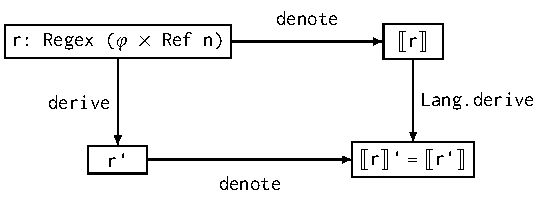
\includegraphics[]{graphics/diagram/diagram.pdf}
\end{center}
\caption{Commuting Square}
\Description[Short Summary]{Long Detailed Description} %% TODO Add a better description
\label{figure_square}
\end{figure}

Second, the derivative algorithm satisfies the commuting square shown in \Cref{figure_square}.
This is proven using the following theorem:
\begin{lstlisting}[label=theorem derive_commutes]
theorem derive_commutes (G: Grammar n φ) Φ [DecidableRel Φ]
  (r: Regex (φ × Ref n)) (node: Node α):
  Rule.denote G Φ (derive G (decideRel Φ) r node)
  = Lang.derive (Rule.denote G Φ r) node
\end{lstlisting}
Note that we use \decideRel to convert a decidable relation that returns a property to a decidable predicate that returns a boolean:
\begin{lstlisting}[label=def decideRel]
def decideRel (p : α → β → Prop) [DecidableRel p]: α → β → Bool :=
  fun a b => decide (p a b)
\end{lstlisting}
We prove that the derivative and denotation squares commute for both the JSONmembers and Katydid algorithms, which implies that validation and filtering proofs follow for each algorithm, including the memoized Katydid algorithm, \refcode{theorem memoize_mem_filter}.

We first verify \TheoremDeriveCommutes for \JSONmembersRuleDerive.
The proof begins with functional induction on \JSONmembersRuleDerive, producing an inductive hypothesis applicable to the symbol case.
All cases are trivial except for the symbol case, where we additionally perform induction on the children and apply the functional inductive hypothesis.

Next, we prove \TheoremDeriveCommutes for \GrammarKatydidDerive.
For each operator except \lstinline{symbol}, we complete the proof by induction on the regular expression, undoing the partial application of the \Node, permuting the parameters, and applying \refcode{theorem Regex.Katydid.derive_is_Regex_derive}, which establishes the equivalence of \RegexKatydidDerive and \RegexDerive:
\begin{lstlisting}[label=theorem Regex.Katydid.derive_is_Regex_derive]
theorem Regex.Katydid.derive_is_Regex_derive (Φ: σ → α → Bool) (r: Regex σ) a:
  Regex.Katydid.derive (flip Φ a) r = Regex.derive Φ r a
\end{lstlisting}
This is proven by \refcode{theorem extract_replace_is_map} and \refcode{theorem regex_derive_is_point_derive}.

The symbol case needs extra work.
As in the proof of \TheoremDeriveCommutes for \JSONmembersRuleDerive, we also need to do two inductions, one for the \Grammar and one for the \Hedge.
Unlike the JSONmembers algorithm's proof, we cannot apply functional induction to a recursive closure, and therefore lack an inductive hypothesis in the \lstinline{symbol} case.
The proof proceeds by applying induction on the children, followed by applying well-founded induction using recursive calls to \TheoremDeriveCommutes.

\subsection{Reflections on the Proof}

The proof relies on two key observations: first, that the algorithm on regular hedge grammars can be generalized to regular expressions via a recursive predicate closure; and second, that the algorithm as a whole amounts to a map operation, up to the final derivative step.

The remainder of the proof is complicated by termination arguments.
We avoided a termination proof for \GrammarKatydidDerive by partially applying the \Node parameter, but termination proofs were required for \RuleDenote in the \lstinline{star} case and \TheoremDeriveCommutes for \GrammarKatydidDerive in the \lstinline{symbol} case.
In \RuleDenote we needed to use a \lstinline{match} expression instead of an \lstinline{∃} operator for termination proof purposes, where \lstinline{∃} would have been more appropriate for a denotation function.

We attempted several versions of the proof before learning how to properly unfold, simplify and prove termination of the recursive closure.
The most intricate part was the termination proof of \TheoremDeriveCommutes for \GrammarKatydidDerive, which relied on the size of the \Node decreasing.
We had to redeclare the well-founded induction call using a membership relation: \lstinline{fun r' x (hx: x ∈ children) => derive_commutes G Φ r' x}.
This gave us the hypothesis we needed to prove termination.

We encountered a similar termination issue when propagating memoization soundness, which required redefining \lstinline{List.foldlM} to both propagate soundness and track that each child is an element of the children list.

\section{Golang implementation}
\label{section_go}

The Katydid memoization technique was originally implemented in Golang in 2016 to filter through petabytes of serialized Protocol Buffers in a proprietary distributed database.
In the previous section, we verified the memoization technique for regular hedge grammars.
In this section, we continue to use Lean as pseudo-code to explain the Go implementation.
The Golang implementation includes several extensions and optimizations beyond the verified technique.
The extensions include a comprehensive predicate library.
The optimizations include smart constructors that simplify regular expressions and compute nullability and hashes for comparisons. 

A significant addition is that instead of parsing the serialized data into a \Hedge data structure in memory, we use a pull-based parser, which only parses what is required and avoids allocating memory on the heap.
The parser is an online parser and therefore performs no backtracking, requiring the order of \Hedge traversal to be refactored.
The predicate and memoized functions (\enter and \leave) are adjusted to operate on a Vector of \Rule rather than a single \Rule, to accommodate the revised traversal order.
We include several implementations of this pull-based parser interface: JSON, Protocol Buffers and one for reflected Go structures, as an option for handling deserialized JSON in the JSONSchema benchmarks.

We include two implementations of the Katydid algorithm: \emph{mem} and \emph{auto}.
The \emph{mem} version of the algorithm, memoizes as the regular hedge grammar is exercised. 
The \emph{auto} version of the algorithm prepopulates the memoization tables with all possibilities.
The auto version adds one more optimization where it finds all constant strings in the predicates and creates another table from these strings to the child expressions, see \link{childr}{def Grammar.Katydid.derive}.

\subsection{Resource-Effectiveness of our Golang implementation}

We conducted benchmarks over several iterations to evaluate how memoization improves filter efficiency with repeated execution.
Two regular hedge grammars (\lstinline{simple} and \lstinline{complex}) were chosen to filter a list of conferences:
\begin{lstlisting}
def simple: Grammar 2 (Pred String) :=
  mk (field ("Category", 1)) #v[emptystr, eq ("Computer Science", 0)]
def complex: Grammar 7 (Pred String) :=
  mk (interleave (eq ("Due", 1)) (interleave (eq ("Loc", 5)) starAny)) #v[emptystr,
    or (field ("Year", 2)) (and (field ("Year", 3)) (field ("Month", 4))),
    eq ("2026", 0), eq ("2025", 0), symbol (Pred.ge "10", 0),
    field ("Cont", 6), eq ("EU", 0),
  ]
def eq (v: α × Fin n) := symbol (Pred.eq v.1, v.2)
def field (v: α × Fin n) := contains (symbol (Pred.eq v.1, v.2))
\end{lstlisting}
The \lstinline{simple} grammar filters for conferences within the Category of Computer Science, while the \lstinline{complex} grammar filters for conferences that have submission deadlines in 2026 or after October 2025 and are also located on the continent of Europe.
For each grammar, we randomly populated data structures and serialized them as Protocol Buffers and JSON.
We ran the benchmarks using Golang version 1.24 on a 2024 MacBook Pro M4 with 48 GB of memory.
Note, we also ran benchmarks back in 2016 and achieved similar sub microsecond results for similar grammars on older hardware.
The supplementary material includes more extensive and larger benchmarks, recorded runs, and explains how to reproduce the benchmarks.

\begin{figure}[t]
\begin{center}
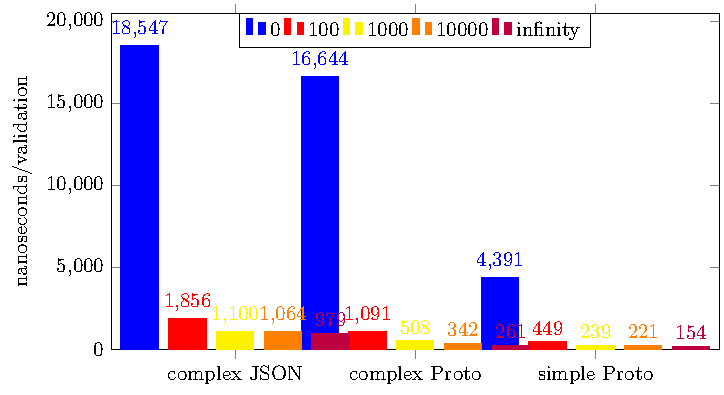
\includegraphics[]{graphics/bargraph/bargraph.pdf}
\caption{Benchmarks}
\Description[Short Summary]{Long Detailed Description} %% TODO Add a better description
\label{figure_benchmarks}
\end{center}
\end{figure}

The results of the benchmarks are shown in \Cref{figure_benchmarks}.
We ran each grammar for multiple iterations.
Zero iterations correspond to no memoization, while infinitely many iterations correspond to fully memoized \enter and \leave functions, with all possible cases precomputed. 
For the other iterations, we recorded the average running time, while memoizing for that number of iterations.
We observe that the longer the same grammar is memoized, the faster the algorithm becomes.
Once the functions are fully memoized over all possible cases, the benchmarks indicate zero heap allocations.
Notice that the JSON benchmarks are slower than the Protocol Buffer benchmarks for the same \lstinline{complex} grammar.
This shift occurs because Protocol Buffers offer superior parsing speeds; our profiling confirms that parsing has become the primary CPU bottleneck.

\subsection{Supporting JSONSchema}

We benchmark our algorithm against other JSONSchema libraries.
For this purpose we implement a translation algorithm from JSONSchema to regular hedge grammars.
Translation is possible, except for a few non-regular operators: \lstinline{uniqueItems} and newer dynamic operators.
%% TODO Walter: be specific about which dynamic operators.
\citet{holstege2019application} explains how JSONSchema can be converted to a \emph{tagged-type regular expressions}, which is closely enough related to regular hedge grammars, that we could apply most of the same translation techniques.

The following JSON: \lstinline[language=json]|{"a": ["b", "c"]}| is represented as the following \Hedge, abstracted away behind a performant pull-based parser: 
\begin{lstlisting}
[node (tag "object") [
   node (string "a") [
     node (tag "array") [
       node (int64 0) [node (string "b") []], node (int64 1) [node (string "c") []]]]]]
\end{lstlisting}
The objects and arrays are tagged with labels to help us support JSONSchema's \lstinline[language=json]|{"type": "object"}| and \lstinline[language=json]|{"type": "array"}|, the arrays are indexed, which makes them handle similar to objects with field names and finally the \Hedge is parameterized over the \Token type:
\begin{lstlisting}[label=Token]
inductive Token where
  | null | bool (value: Bool) | string (value: String) | tag (value: String)
  | int64 (value: Int64) | float64 (value: Float64Bits) | decimal (value: String) | ...
\end{lstlisting}
This includes several representations of numbers for optimization purposes, as well as to generically support other serialization formats.

We can translate the \jsonlink{"small jsonschema for a blogpost"}{jsonschema_blogpost} to a regular hedge grammar:
\begin{lstlisting}
def example_tagged_grammar_blogpost : Grammar 7 JSONSchema.Pred := Grammar.mk
  (start := (symbol (Pred.tagEq "object", 4)))
  (prods := #v[emptystr, starAny, symbol (Pred.string, 0), symbol (Pred.email, 0),
               (interleave (symbol (Pred.strEq "content", 2))
                           (symbol (Pred.strEq "author", 5))),
               (symbol (Pred.tagEq "object", 6)),
               (interleave (symbol (Pred.strEq "username", 2))
                          (optional (symbol (Pred.strEq "email", 3))))])
\end{lstlisting}
%% TODO Walter: Check this is actually what the schema is translated to ^^

Most operators translate seamlessly, for example \lstinline[language=json]|"anyOf"|, \lstinline[language=json]|"allOf"| and \lstinline[language=json]|"not"|, while others
posed a challenge, for example \lstinline[language=json]|"dependentRequired"|, overlapping \lstinline[language=json]|"patternProperties"| and \lstinline[language=json]|"additionalProperties"|.
For example, if the \lstinline[language=json]|"additionalProperties"| field is not set, it defaults to true, which means other fields are allowed, so we need to add an extra constraint, that match any fields that were not already defined:
\begin{lstlisting}
star (symbol (Pred.not (Pred.or (Pred.strEq "content") (Pred.strEq "author"))), 1))
\end{lstlisting}
%% TODO Walter: Check this is actually what the schema is translated to ^^

We tested our translation against the JSONSchema testsuite for \verb+draft4+ and the newest \verb+version 2020-12+, where we pass all tests (1386 out of 2000) except those that include features that are not regular: \lstinline{uniqueItems}, dynamicAnchor, remoteRef.
%% TODO Walter: Make sure this is the complete list ^^ of unsupported features.
%% TODO Walter: Put in the actual numbers and how many tests we skipped because of unsupported features.

\section{Benchmarks}
\label{section_benchmarks}

Our JSONSchema benchmark extends the suite developed by \citet{blaze}. In the following sections, we detail the underlying implementations, schemas, and measurement methodologies.

The benchmarks include many implementations in various programming languages.
% We added the following third-party libraries:
% rapidjson~\cite{jsonschema_impl_rapidjson} (C++),
% go-google~\cite{jsonschema_impl_go-google} (Golang),
% go-json-schema-spec~\cite{jsonschema_impl_go-json-schema-spec} (Golang),
% go-kaptinlin~\cite{jsonschema_impl_go-kaptinlin} (Golang).
% The benchmark suite includes alternative Go libraries as well as an event-based C++ parser to serve as baselines for our pull-based implementation.
For brevity, we restrict our discussion to the fastest implementations:
\begin{itemize}
\item ajv-bun~\cite{jsonschema_impl_ajv} (Javascript executed on the BUN~\cite{javascript_engine_bun} engine),
\item blaze~\cite{blaze} (C++),
\item boon~\cite{jsonschema_impl_boon} (Rust),
\item go-santhosh-tekuri~\cite{jsonschema_impl_go-santhosh-tekuri} (Golang),
\item jsu-c~\cite{jsonschema_impl_jsu} (generated C),
\item and katydid (Golang).
\end{itemize}
To avoid redundancy, we highlight only the optimal variants from the ajv and jsu families.
While go-santhosh-tekuri was the most efficient external Go library, katydid demonstrated superior performance across all Go-centric evaluations.
We also evaluate four variants of our Katydid framework, differentiated by their memoization strategy (on-the-fly vs. prepopulated) and parsing target (online JSON vs. Go reflection): go-katydid-mem-json, go-katydid-auto-json, go-katydid-mem-reflect, and go-katydid-auto-reflect.
To guarantee cross-platform portability and reproducibility, each configuration is packaged with a dedicated Docker setup.

% The original benchmark suite included the following implementations: 
% ajv~\cite{jsonschema_impl_ajv} (Javascript),
% ajv-bun~\cite{jsonschema_impl_ajv} (Javascript executed on the BUN~\cite{javascript_engine_bun} engine),
% blaze~\cite{blaze} (C++),
% boon~\cite{jsonschema_impl_boon} (Rust),
% corvus~\cite{jsonschema_impl_corvus} (generated C\#),
% go-santhosh-tekuri~\cite{jsonschema_impl_go-santhosh-tekuri} (Golang),
% hyperjump~\cite{jsonschema_impl_hyperjump} (Javascript),
% jsdotnet~\cite{jsonschema_impl_jsdotnet} (C\#),
% json\_schemer~\cite{jsonschema_impl_json_schemer} (Ruby),
% jsoncons~\cite{jsonschema_impl_jsoncons} (C++),
% jsu-c~\cite{jsonschema_impl_jsu} (generated C),
% jsu-java~\cite{jsonschema_impl_jsu} (generated Java),
% jsu-js~\cite{jsonschema_impl_jsu} (generated Javascript),
% jsu-pl~\cite{jsonschema_impl_jsu} (generated Perl),
% jsu-py~\cite{jsonschema_impl_jsu} (generated Python),
% JSV~\cite{jsonschema_impl_JSV} (Elixir),
% kmp~\cite{jsonschema_impl_kmp} (Kotlin),
% networknt~\cite{jsonschema_impl_networknt} (Java)
% opis~\cite{jsonschema_impl_opis} (PHP),
% py-jsonschema~\cite{jsonschema_impl_py-jsonschema} (Python),
% schemasafe~\cite{jsonschema_impl_schemasafe} (Javascript).

\citet{blaze} collected schemas from the JSONSchema Store~\cite{schemastore} and then crawled GitHub for valid JSON documents for each of these schemas.
% :
% ansible-meta,
% aws-cdk,
% babelrc,
% clang-format,
% cmake-presets,
% code-climate,
% cql2,
% cspell,
% cypress,
% deno,
% dependabot,
% draft-04,
% fabric-mod,
% geojson,
% gitpod-configuration,
% helm-chart-lock,
% importmap,
% jasmine,
% jsconfig,
% jshintrc,
% krakend,
% lazygit,
% lerna,
% nest-cli,
% omnisharp,
% openapi,
% pre-commit-hooks,
% pulumi,
% semantic-release,
% stale,
% stylecop,
% tmuxinator,
% ui5,
% ui5-manifest,
% unreal-engine-uproject,
% vercel,
% yamllint.
We add schemas from the official JSONSchema examples~\cite{jsonschemaexamples}.
% :
% address,
% blogpost,
% calendar,
% devicetype,
% health-record,
% job-posting,
% movie,
% userprofile.
We also add schemas from ajv's benchmarks.
% cosmicrealms~\cite{jsonschema_impl_ajv},
% : 
% complex~\cite{jsonschema_jsck},
% medium~\cite{jsonschema_jsck},
% advanced~\cite{jsonschema_zschema},
% basic~\cite{jsonschema_zschema}.
Finally, we include the JSON schema for the conference example previously introduced.
To evaluate the extended schema collection, we developed a random generator capable of producing both valid instances and non-conforming documents containing at least one schema violation.
For schemas utilizing the \lstinline{uniqueItems} constraint, we derived variants that omit this feature; this allows for isolated benchmarking of the remaining schema logic.
See \Cref{table_jsonschemas} for a summary of the schemas.

\begin{table}
\caption[JSON Schemas used for benchmarks]{JSON Schemas used for benchmarks, where rm indicates that features were removed from the original schema and gen indicates that the documents were generated.}
\label{table_jsonschemas}
%% generate table by running: `make analytics-schemas` in the benchmark suite.
% BEGIN Generated tabular
\begin{tabular}{l|lllll}
name & schema size (B) & \# Docs & avg doc size (B) & gen & rm \\
\hline
cosmicrealms & 1583 & 10000 & 547 & \cmark & \cmark \\
ansible-meta & 37015 & 333 & 312 & \xmark & \xmark \\
aws-cdk & 740 & 483 & 1149 & \xmark & \xmark \\
babelrc & 6717 & 794 & 140 & \xmark & \xmark \\
clang-format & 55557 & 133 & 334 & \xmark & \xmark \\
cmake-presets & 86084 & 967 & 2719 & \xmark & \xmark \\
code-climate & 6051 & 2484 & 281 & \xmark & \xmark \\
cql2 & 18400 & 109 & 124 & \xmark & \xmark \\
cspell & 128640 & 981 & 819 & \xmark & \cmark \\
cypress & 16457 & 981 & 403 & \xmark & \xmark \\
deno & 22822 & 987 & 1022 & \xmark & \cmark \\
dependabot & 9631 & 967 & 403 & \xmark & \xmark \\
draft-04 & 4020 & 563 & 12635 & \xmark & \cmark \\
address & 761 & 10000 & 140 & \cmark & \xmark \\
blogpost & 1265 & 10000 & 328 & \cmark & \xmark \\
calendar & 1499 & 10000 & 341 & \cmark & \xmark \\
devicetype & 1457 & 10000 & 189 & \cmark & \xmark \\
health-record & 1509 & 10000 & 416 & \cmark & \xmark \\
job-posting & 674 & 10000 & 220 & \cmark & \xmark \\
movie & 708 & 10000 & 243 & \cmark & \xmark \\
userprofile & 631 & 10000 & 221 & \cmark & \xmark \\
fabric-mod & 11446 & 911 & 691 & \xmark & \xmark \\
geojson & 46177 & 500 & 52329 & \xmark & \xmark \\
gitpod-configuration & 13489 & 986 & 357 & \xmark & \xmark \\
helm-chart-lock & 1556 & 3888 & 342 & \xmark & \xmark \\
importmap & 618 & 964 & 629 & \xmark & \xmark \\
jasmine & 3690 & 980 & 133 & \xmark & \xmark \\
complex & 4060 & 100 & 31530 & \cmark & \xmark \\
medium & 1887 & 10000 & 365 & \cmark & \xmark \\
jsconfig & 60482 & 981 & 177 & \xmark & \cmark \\
jshintrc & 12142 & 966 & 428 & \xmark & \xmark \\
conf & 1053 & 10000 & 223 & \cmark & \xmark \\
krakend & 372808 & 47 & 2382 & \xmark & \cmark \\
lazygit & 89462 & 280 & 276 & \xmark & \cmark \\
lerna & 4717 & 985 & 173 & \xmark & \xmark \\
nest-cli & 19450 & 1025 & 290 & \xmark & \xmark \\
omnisharp & 13924 & 987 & 595 & \xmark & \xmark \\
openapi & 33281 & 107 & 164593 & \xmark & \xmark \\
pre-commit-hooks & 9920 & 985 & 551 & \xmark & \xmark \\
pulumi & 7983 & 3807 & 251 & \xmark & \xmark \\
semantic-release & 3422 & 794 & 461 & \xmark & \xmark \\
stale & 3702 & 961 & 469 & \xmark & \xmark \\
stylecop & 11732 & 983 & 568 & \xmark & \cmark \\
tmuxinator & 4545 & 382 & 629 & \xmark & \xmark \\
ui5 & 96365 & 942 & 487 & \xmark & \xmark \\
ui5-manifest & 392675 & 611 & 2353 & \xmark & \cmark \\
unreal-engine-uproject & 10402 & 859 & 394 & \xmark & \cmark \\
vercel & 38187 & 710 & 406 & \xmark & \xmark \\
yamllint & 890 & 984 & 352 & \xmark & \xmark \\
advanced & 2618 & 10000 & 366 & \cmark & \cmark \\
basic & 975 & 200 & 2783 & \cmark & \cmark \\
\end{tabular}
% END Generated tabular
\end{table}

While \citet{blaze} accounts for schema compilation time and validation performance in both ``cold'' (unprimed) and ``warm'' (primed) states, we introduce a distinct measurement for parsing time.
This addition underscores that parsing is an integral component of the total validation overhead—a factor that becomes particularly significant when filtering through large volumes of non-matching documents.

Benchmarks were conducted on a 2024 MacBook Pro equipped with an M4 processor and 48 GB of memory.
To ensure statistical stability, each benchmark was executed three times, with results reported as the average execution time.
%% TODO Walter: Actually run it tree times.

\subsection{Results}

\begin{table}
\label{table_jsonschema_results}
\caption{results}

% BEGIN Generated tabular
\begin{tabular}{lll|llll}
name & mixed & impl & \#warm & \%warm & \#cold & \%cold \\
\hline
cosmicrealms & \xmark & ajv-bun & 4 & 300\% & 6 & 892\% \\
cosmicrealms & \xmark & blaze & 5 & 493\% & 4 & 447\% \\
cosmicrealms & \xmark & boon & 6 & 891\% & 5 & 882\% \\
cosmicrealms & \xmark & go-katydid-auto-json & 7 & 3142\% & 7 & 2984\% \\
cosmicrealms & \xmark & go-katydid-auto-reflect & 2 & 160\% & 3 & 206\% \\
cosmicrealms & \xmark & go-katydid-mem-json & 9 & 10255\% & 9 & 35613\% \\
cosmicrealms & \xmark & go-katydid-mem-reflect & 1 & 100\% & 1 & 100\% \\
cosmicrealms & \xmark & go-santhosh-tekuri & 8 & 6697\% & 8 & 5881\% \\
cosmicrealms & \xmark & jsu-c & 3 & 193\% & 2 & 170\% \\
\hline
aws-cdk & \xmark & ajv-bun & 3 & 159\% & 6 & 2054\% \\
aws-cdk & \xmark & blaze & 1 & 100\% & 2 & 176\% \\
aws-cdk & \xmark & boon & 6 & 735\% & 5 & 612\% \\
aws-cdk & \xmark & go-katydid-auto-json & 8 & 8910\% & 8 & 6699\% \\
aws-cdk & \xmark & go-katydid-auto-reflect & 5 & 368\% & 3 & 288\% \\
aws-cdk & \xmark & go-katydid-mem-json & 9 & 9391\% & 9 & 8492\% \\
aws-cdk & \xmark & go-katydid-mem-reflect & 4 & 341\% & 4 & 333\% \\
aws-cdk & \xmark & go-santhosh-tekuri & 7 & 3140\% & 7 & 2640\% \\
aws-cdk & \xmark & jsu-c & 2 & 116\% & 1 & 100\% \\
\hline
babelrc & \xmark & ajv-bun & 3 & 292\% & 7 & 2850\% \\
babelrc & \xmark & blaze & 2 & 111\% & 2 & 107\% \\
babelrc & \xmark & boon & 6 & 851\% & 5 & 451\% \\
babelrc & \xmark & go-katydid-auto-json & 7 & 2350\% & 6 & 1285\% \\
babelrc & \xmark & go-katydid-auto-reflect & 4 & 449\% & 3 & 261\% \\
babelrc & \xmark & go-katydid-mem-json & 9 & 4275\% & 9 & 4924\% \\
babelrc & \xmark & go-katydid-mem-reflect & 5 & 669\% & 4 & 414\% \\
babelrc & \xmark & go-santhosh-tekuri & 8 & 3464\% & 8 & 3049\% \\
babelrc & \xmark & jsu-c & 1 & 100\% & 1 & 100\% \\
\hline
clang-format & \xmark & ajv-bun & 7 & 2347\% & 8 & 28164\% \\
clang-format & \xmark & blaze & 4 & 292\% & 4 & 370\% \\
clang-format & \xmark & boon & 5 & 616\% & 5 & 515\% \\
clang-format & \xmark & go-katydid-auto-json & 6 & 1901\% & 6 & 1394\% \\
clang-format & \xmark & go-katydid-auto-reflect & 2 & 114\% & 1 & 100\% \\
clang-format & \xmark & go-katydid-mem-json & 9 & 20981\% & 9 & 101885\% \\
clang-format & \xmark & go-katydid-mem-reflect & 3 & 124\% & 3 & 162\% \\
clang-format & \xmark & go-santhosh-tekuri & 8 & 2575\% & 7 & 1956\% \\
clang-format & \xmark & jsu-c & 1 & 100\% & 2 & 116\% \\
\hline
cypress & \xmark & ajv-bun & 6 & 725\% & 8 & 4276\% \\
cypress & \xmark & blaze & 1 & 100\% & 2 & 133\% \\
cypress & \xmark & boon & 5 & 457\% & 5 & 358\% \\
cypress & \xmark & go-katydid-auto-json & 8 & 3372\% & 7 & 2675\% \\
cypress & \xmark & go-katydid-auto-reflect & 3 & 211\% & 3 & 169\% \\
cypress & \xmark & go-katydid-mem-json & 9 & 10092\% & 9 & 11792\% \\
cypress & \xmark & go-katydid-mem-reflect & 4 & 284\% & 4 & 205\% \\
cypress & \xmark & go-santhosh-tekuri & 7 & 1260\% & 6 & 1410\% \\
cypress & \xmark & jsu-c & 2 & 108\% & 1 & 100\% \\
\hline
deno & \xmark & ajv-bun & 5 & 456\% & 7 & 2198\% \\
deno & \xmark & blaze & 2 & 107\% & 4 & 206\% \\
deno & \xmark & boon & 6 & 516\% & 5 & 439\% \\
deno & \xmark & go-katydid-auto-json & 8 & 4061\% & 8 & 2833\% \\
deno & \xmark & go-katydid-auto-reflect & 3 & 140\% & 2 & 118\% \\
deno & \xmark & go-katydid-mem-json & 9 & 7281\% & 9 & 4572\% \\
deno & \xmark & go-katydid-mem-reflect & 4 & 145\% & 3 & 140\% \\
deno & \xmark & go-santhosh-tekuri & 7 & 1877\% & 6 & 1192\% \\
deno & \xmark & jsu-c & 1 & 100\% & 1 & 100\% \\
\hline
dependabot & \xmark & ajv-bun & 5 & 186\% & 6 & 1333\% \\
dependabot & \xmark & blaze & 3 & 126\% & 4 & 208\% \\
dependabot & \xmark & boon & 6 & 731\% & 5 & 719\% \\
dependabot & \xmark & go-katydid-auto-json & 7 & 2582\% & 7 & 2285\% \\
dependabot & \xmark & go-katydid-auto-reflect & 4 & 168\% & 1 & 100\% \\
dependabot & \xmark & go-katydid-mem-json & 9 & 4833\% & 9 & 4917\% \\
dependabot & \xmark & go-katydid-mem-reflect & 1 & 100\% & 2 & 103\% \\
dependabot & \xmark & go-santhosh-tekuri & 8 & 2954\% & 8 & 2734\% \\
dependabot & \xmark & jsu-c & 2 & 123\% & 3 & 162\% \\
\hline
address & \xmark & ajv-bun & 2 & 119\% & 5 & 314\% \\
address & \xmark & blaze & 1 & 100\% & 1 & 100\% \\
address & \xmark & boon & 6 & 426\% & 6 & 362\% \\
address & \xmark & go-katydid-auto-json & 7 & 1202\% & 7 & 983\% \\
address & \xmark & go-katydid-auto-reflect & 3 & 136\% & 2 & 121\% \\
address & \xmark & go-katydid-mem-json & 9 & 3087\% & 9 & 2954\% \\
address & \xmark & go-katydid-mem-reflect & 5 & 242\% & 3 & 127\% \\
address & \xmark & go-santhosh-tekuri & 8 & 1232\% & 8 & 1023\% \\
address & \xmark & jsu-c & 4 & 226\% & 4 & 190\% \\
\hline
blogpost & \xmark & ajv-bun & 5 & 137\% & 5 & 427\% \\
blogpost & \xmark & blaze & 4 & 136\% & 4 & 206\% \\
blogpost & \xmark & boon & 6 & 477\% & 6 & 548\% \\
blogpost & \xmark & go-katydid-auto-json & 7 & 1598\% & 7 & 1697\% \\
blogpost & \xmark & go-katydid-auto-reflect & 1 & 100\% & 3 & 128\% \\
blogpost & \xmark & go-katydid-mem-json & 9 & 2622\% & 9 & 2759\% \\
blogpost & \xmark & go-katydid-mem-reflect & 2 & 106\% & 1 & 100\% \\
blogpost & \xmark & go-santhosh-tekuri & 8 & 2193\% & 8 & 2402\% \\
blogpost & \xmark & jsu-c & 3 & 108\% & 2 & 124\% \\
\hline
calendar & \xmark & ajv-bun & 4 & 164\% & 5 & 404\% \\
calendar & \xmark & blaze & 5 & 182\% & 4 & 241\% \\
calendar & \xmark & boon & 6 & 430\% & 6 & 446\% \\
calendar & \xmark & go-katydid-auto-json & 7 & 1383\% & 7 & 1329\% \\
calendar & \xmark & go-katydid-auto-reflect & 3 & 130\% & 3 & 133\% \\
calendar & \xmark & go-katydid-mem-json & 9 & 3237\% & 9 & 3061\% \\
calendar & \xmark & go-katydid-mem-reflect & 2 & 103\% & 2 & 107\% \\
calendar & \xmark & go-santhosh-tekuri & 8 & 1918\% & 8 & 1879\% \\
calendar & \xmark & jsu-c & 1 & 100\% & 1 & 100\% \\
\hline
devicetype & \xmark & ajv-bun & 2 & 121\% & 5 & 530\% \\
devicetype & \xmark & blaze & 1 & 100\% & 1 & 100\% \\
devicetype & \xmark & boon & 6 & 995\% & 6 & 831\% \\
devicetype & \xmark & go-katydid-auto-json & 7 & 1129\% & 7 & 909\% \\
devicetype & \xmark & go-katydid-auto-reflect & 5 & 179\% & 3 & 145\% \\
devicetype & \xmark & go-katydid-mem-json & 8 & 2687\% & 8 & 2423\% \\
devicetype & \xmark & go-katydid-mem-reflect & 4 & 164\% & 4 & 148\% \\
devicetype & \xmark & go-santhosh-tekuri & 9 & 2927\% & 9 & 2473\% \\
devicetype & \xmark & jsu-c & 3 & 127\% & 2 & 106\% \\
\hline
health-record & \xmark & ajv-bun & 4 & 193\% & 5 & 543\% \\
health-record & \xmark & blaze & 5 & 221\% & 4 & 281\% \\
health-record & \xmark & boon & 6 & 711\% & 6 & 714\% \\
health-record & \xmark & go-katydid-auto-json & 7 & 2439\% & 7 & 2245\% \\
health-record & \xmark & go-katydid-auto-reflect & 2 & 118\% & 3 & 171\% \\
health-record & \xmark & go-katydid-mem-json & 9 & 3582\% & 9 & 3409\% \\
health-record & \xmark & go-katydid-mem-reflect & 1 & 100\% & 1 & 100\% \\
health-record & \xmark & go-santhosh-tekuri & 8 & 3012\% & 8 & 2959\% \\
health-record & \xmark & jsu-c & 3 & 154\% & 2 & 155\% \\
\hline
job-posting & \xmark & ajv-bun & 2 & 149\% & 5 & 440\% \\
job-posting & \xmark & blaze & 3 & 157\% & 4 & 177\% \\
job-posting & \xmark & boon & 6 & 438\% & 6 & 452\% \\
job-posting & \xmark & go-katydid-auto-json & 7 & 1463\% & 7 & 1436\% \\
job-posting & \xmark & go-katydid-auto-reflect & 4 & 163\% & 2 & 166\% \\
job-posting & \xmark & go-katydid-mem-json & 9 & 2586\% & 9 & 2658\% \\
job-posting & \xmark & go-katydid-mem-reflect & 5 & 307\% & 3 & 176\% \\
job-posting & \xmark & go-santhosh-tekuri & 8 & 1746\% & 8 & 1838\% \\
job-posting & \xmark & jsu-c & 1 & 100\% & 1 & 100\% \\
\hline
movie & \xmark & ajv-bun & 3 & 135\% & 5 & 413\% \\
movie & \xmark & blaze & 2 & 132\% & 4 & 166\% \\
movie & \xmark & boon & 6 & 444\% & 6 & 442\% \\
movie & \xmark & go-katydid-auto-json & 7 & 1525\% & 7 & 1482\% \\
movie & \xmark & go-katydid-auto-reflect & 4 & 154\% & 3 & 156\% \\
movie & \xmark & go-katydid-mem-json & 9 & 2603\% & 9 & 2520\% \\
movie & \xmark & go-katydid-mem-reflect & 5 & 155\% & 2 & 152\% \\
movie & \xmark & go-santhosh-tekuri & 8 & 1619\% & 8 & 1674\% \\
movie & \xmark & jsu-c & 1 & 100\% & 1 & 100\% \\
\hline
userprofile & \xmark & ajv-bun & 3 & 127\% & 5 & 394\% \\
userprofile & \xmark & blaze & 2 & 118\% & 2 & 156\% \\
userprofile & \xmark & boon & 6 & 426\% & 6 & 691\% \\
userprofile & \xmark & go-katydid-auto-json & 7 & 1533\% & 7 & 1538\% \\
userprofile & \xmark & go-katydid-auto-reflect & 4 & 165\% & 4 & 172\% \\
userprofile & \xmark & go-katydid-mem-json & 9 & 2552\% & 9 & 2490\% \\
userprofile & \xmark & go-katydid-mem-reflect & 5 & 169\% & 3 & 161\% \\
userprofile & \xmark & go-santhosh-tekuri & 8 & 2261\% & 8 & 2126\% \\
userprofile & \xmark & jsu-c & 1 & 100\% & 1 & 100\% \\
\hline
fabric-mod & \xmark & ajv-bun & 5 & 683\% & 7 & 4064\% \\
fabric-mod & \xmark & blaze & 4 & 294\% & 4 & 322\% \\
fabric-mod & \xmark & boon & 6 & 1405\% & 5 & 1637\% \\
fabric-mod & \xmark & go-katydid-auto-json & 7 & 3201\% & 6 & 2828\% \\
fabric-mod & \xmark & go-katydid-auto-reflect & 2 & 107\% & 1 & 100\% \\
fabric-mod & \xmark & go-katydid-mem-json & 9 & 8380\% & 9 & 8059\% \\
fabric-mod & \xmark & go-katydid-mem-reflect & 1 & 100\% & 2 & 118\% \\
fabric-mod & \xmark & go-santhosh-tekuri & 8 & 8133\% & 8 & 5923\% \\
fabric-mod & \xmark & jsu-c & 3 & 166\% & 3 & 154\% \\
\hline
gitpod-configuration & \xmark & ajv-bun & 5 & 486\% & 9 & 2916\% \\
gitpod-configuration & \xmark & blaze & 2 & 104\% & 4 & 184\% \\
gitpod-configuration & \xmark & boon & 6 & 523\% & 5 & 447\% \\
gitpod-configuration & \xmark & go-katydid-auto-json & 7 & 1971\% & 7 & 1640\% \\
gitpod-configuration & \xmark & go-katydid-auto-reflect & 4 & 151\% & 2 & 116\% \\
gitpod-configuration & \xmark & go-katydid-mem-json & 9 & 2607\% & 8 & 2626\% \\
gitpod-configuration & \xmark & go-katydid-mem-reflect & 3 & 143\% & 3 & 127\% \\
gitpod-configuration & \xmark & go-santhosh-tekuri & 8 & 2065\% & 6 & 1589\% \\
gitpod-configuration & \xmark & jsu-c & 1 & 100\% & 1 & 100\% \\
\hline
helm-chart-lock & \xmark & ajv-bun & 2 & 248\% & 5 & 552\% \\
helm-chart-lock & \xmark & blaze & 1 & 100\% & 1 & 100\% \\
helm-chart-lock & \xmark & boon & 6 & 1987\% & 6 & 577\% \\
helm-chart-lock & \xmark & go-katydid-auto-json & 8 & 7041\% & 8 & 1897\% \\
helm-chart-lock & \xmark & go-katydid-auto-reflect & 4 & 558\% & 3 & 155\% \\
helm-chart-lock & \xmark & go-katydid-mem-json & 9 & 8066\% & 9 & 2261\% \\
helm-chart-lock & \xmark & go-katydid-mem-reflect & 5 & 1585\% & 4 & 168\% \\
helm-chart-lock & \xmark & go-santhosh-tekuri & 7 & 6411\% & 7 & 1732\% \\
helm-chart-lock & \xmark & jsu-c & 3 & 377\% & 2 & 132\% \\
\hline
importmap & \xmark & ajv-bun & 3 & 470\% & 6 & 2115\% \\
importmap & \xmark & blaze & 1 & 100\% & 1 & 100\% \\
importmap & \xmark & boon & 6 & 2139\% & 5 & 1043\% \\
importmap & \xmark & go-katydid-auto-json & 9 & 10247\% & 8 & 4712\% \\
importmap & \xmark & go-katydid-auto-reflect & 5 & 688\% & 3 & 342\% \\
importmap & \xmark & go-katydid-mem-json & 8 & 9812\% & 9 & 5189\% \\
importmap & \xmark & go-katydid-mem-reflect & 4 & 672\% & 4 & 349\% \\
importmap & \xmark & go-santhosh-tekuri & 7 & 7044\% & 7 & 4186\% \\
importmap & \xmark & jsu-c & 2 & 382\% & 2 & 185\% \\
\hline
jasmine & \xmark & ajv-bun & 3 & 126\% & 6 & 1603\% \\
jasmine & \xmark & blaze & 2 & 107\% & 2 & 131\% \\
jasmine & \xmark & boon & 6 & 986\% & 4 & 748\% \\
jasmine & \xmark & go-katydid-auto-json & 7 & 2111\% & 7 & 1613\% \\
jasmine & \xmark & go-katydid-auto-reflect & 5 & 291\% & 3 & 246\% \\
jasmine & \xmark & go-katydid-mem-json & 9 & 4873\% & 9 & 4149\% \\
jasmine & \xmark & go-katydid-mem-reflect & 4 & 279\% & 5 & 1244\% \\
jasmine & \xmark & go-santhosh-tekuri & 8 & 3613\% & 8 & 2820\% \\
jasmine & \xmark & jsu-c & 1 & 100\% & 1 & 100\% \\
\hline
complex & \xmark & ajv-bun & 5 & 131872\% & 6 & 94552\% \\
complex & \xmark & blaze & 4 & 81176\% & 4 & 26684\% \\
complex & \xmark & boon & 6 & 180881\% & 5 & 71713\% \\
complex & \xmark & go-katydid-auto-json & 7 & 555231\% & 7 & 183865\% \\
complex & \xmark & go-katydid-auto-reflect & 1 & 100\% & 2 & 143\% \\
complex & \xmark & go-katydid-mem-json & 8 & 628881\% & 8 & 218982\% \\
complex & \xmark & go-katydid-mem-reflect & 2 & 771\% & 1 & 100\% \\
complex & \xmark & go-santhosh-tekuri & 9 & 1103005\% & 9 & 359602\% \\
complex & \xmark & jsu-c & 3 & 54782\% & 3 & 19195\% \\
\hline
medium & \xmark & ajv-bun & 1 & 100\% & 5 & 227\% \\
medium & \xmark & blaze & 5 & 240\% & 3 & 177\% \\
medium & \xmark & boon & 6 & 763\% & 6 & 506\% \\
medium & \xmark & go-katydid-auto-json & 7 & 2173\% & 7 & 1108\% \\
medium & \xmark & go-katydid-auto-reflect & 3 & 127\% & 2 & 115\% \\
medium & \xmark & go-katydid-mem-json & 9 & 2897\% & 9 & 1466\% \\
medium & \xmark & go-katydid-mem-reflect & 2 & 116\% & 4 & 177\% \\
medium & \xmark & go-santhosh-tekuri & 8 & 2767\% & 8 & 1459\% \\
medium & \xmark & jsu-c & 4 & 159\% & 1 & 100\% \\
\hline
jsconfig & \xmark & ajv-bun & 6 & 775\% & 8 & 2162\% \\
jsconfig & \xmark & blaze & 1 & 100\% & 2 & 112\% \\
jsconfig & \xmark & boon & 5 & 746\% & 5 & 605\% \\
jsconfig & \xmark & go-katydid-auto-json & 7 & 1351\% & 6 & 848\% \\
jsconfig & \xmark & go-katydid-auto-reflect & 3 & 169\% & 3 & 117\% \\
jsconfig & \xmark & go-katydid-mem-json & 9 & 6586\% & 9 & 9083\% \\
jsconfig & \xmark & go-katydid-mem-reflect & 4 & 603\% & 4 & 388\% \\
jsconfig & \xmark & go-santhosh-tekuri & 8 & 2693\% & 7 & 1951\% \\
jsconfig & \xmark & jsu-c & 2 & 125\% & 1 & 100\% \\
\hline
jshintrc & \xmark & ajv-bun & 6 & 599\% & 6 & 1589\% \\
jshintrc & \xmark & blaze & 4 & 353\% & 4 & 364\% \\
jshintrc & \xmark & boon & 5 & 543\% & 5 & 594\% \\
jshintrc & \xmark & go-katydid-auto-json & 8 & 11174\% & 8 & 9413\% \\
jshintrc & \xmark & go-katydid-auto-reflect & 1 & 100\% & 1 & 100\% \\
jshintrc & \xmark & go-katydid-mem-json & 9 & 25779\% & 9 & 24045\% \\
jshintrc & \xmark & go-katydid-mem-reflect & 2 & 104\% & 2 & 108\% \\
jshintrc & \xmark & go-santhosh-tekuri & 7 & 2043\% & 7 & 2125\% \\
jshintrc & \xmark & jsu-c & 3 & 147\% & 3 & 151\% \\
\hline
conf & \xmark & ajv-bun & 2 & 102\% & 5 & 288\% \\
conf & \xmark & blaze & 1 & 100\% & 3 & 150\% \\
conf & \xmark & boon & 6 & 901\% & 6 & 742\% \\
conf & \xmark & go-katydid-auto-json & 7 & 1930\% & 7 & 1424\% \\
conf & \xmark & go-katydid-auto-reflect & 4 & 132\% & 2 & 136\% \\
conf & \xmark & go-katydid-mem-json & 8 & 2172\% & 8 & 1636\% \\
conf & \xmark & go-katydid-mem-reflect & 3 & 116\% & 1 & 100\% \\
conf & \xmark & go-santhosh-tekuri & 9 & 2352\% & 9 & 1792\% \\
conf & \xmark & jsu-c & 5 & 153\% & 4 & 241\% \\
\hline
lazygit & \xmark & ajv-bun & 6 & 1386\% & 9 & 16600\% \\
lazygit & \xmark & blaze & 4 & 142\% & 4 & 282\% \\
lazygit & \xmark & boon & 5 & 757\% & 5 & 689\% \\
lazygit & \xmark & go-katydid-auto-json & 7 & 1861\% & 6 & 1515\% \\
lazygit & \xmark & go-katydid-auto-reflect & 3 & 105\% & 1 & 100\% \\
lazygit & \xmark & go-katydid-mem-json & 9 & 4335\% & 8 & 11358\% \\
lazygit & \xmark & go-katydid-mem-reflect & 2 & 101\% & 2 & 105\% \\
lazygit & \xmark & go-santhosh-tekuri & 8 & 2541\% & 7 & 2344\% \\
lazygit & \xmark & jsu-c & 1 & 100\% & 3 & 123\% \\
\hline
lerna & \xmark & ajv-bun & 3 & 205\% & 6 & 1246\% \\
lerna & \xmark & blaze & 1 & 100\% & 2 & 184\% \\
lerna & \xmark & boon & 6 & 512\% & 5 & 434\% \\
lerna & \xmark & go-katydid-auto-json & 8 & 2354\% & 8 & 2083\% \\
lerna & \xmark & go-katydid-auto-reflect & 5 & 248\% & 3 & 192\% \\
lerna & \xmark & go-katydid-mem-json & 9 & 3432\% & 9 & 2690\% \\
lerna & \xmark & go-katydid-mem-reflect & 4 & 244\% & 4 & 192\% \\
lerna & \xmark & go-santhosh-tekuri & 7 & 1932\% & 7 & 1550\% \\
lerna & \xmark & jsu-c & 2 & 101\% & 1 & 100\% \\
\hline
nest-cli & \xmark & ajv-bun & 5 & 305\% & 7 & 1524\% \\
nest-cli & \xmark & blaze & 1 & 100\% & 3 & 112\% \\
nest-cli & \xmark & boon & 6 & 754\% & 5 & 540\% \\
nest-cli & \xmark & go-katydid-auto-json & 7 & 2401\% & 6 & 1307\% \\
nest-cli & \xmark & go-katydid-auto-reflect & 4 & 180\% & 2 & 110\% \\
nest-cli & \xmark & go-katydid-mem-json & 9 & 3732\% & 9 & 2485\% \\
nest-cli & \xmark & go-katydid-mem-reflect & 3 & 176\% & 4 & 124\% \\
nest-cli & \xmark & go-santhosh-tekuri & 8 & 2569\% & 8 & 1551\% \\
nest-cli & \xmark & jsu-c & 2 & 122\% & 1 & 100\% \\
\hline
omnisharp & \xmark & ajv-bun & 5 & 380\% & 7 & 1755\% \\
omnisharp & \xmark & blaze & 4 & 201\% & 3 & 264\% \\
omnisharp & \xmark & boon & 6 & 565\% & 5 & 700\% \\
omnisharp & \xmark & go-katydid-auto-json & 8 & 2951\% & 8 & 2629\% \\
omnisharp & \xmark & go-katydid-auto-reflect & 2 & 116\% & 4 & 495\% \\
omnisharp & \xmark & go-katydid-mem-json & 9 & 14109\% & 9 & 14988\% \\
omnisharp & \xmark & go-katydid-mem-reflect & 3 & 123\% & 2 & 116\% \\
omnisharp & \xmark & go-santhosh-tekuri & 7 & 1798\% & 6 & 1578\% \\
omnisharp & \xmark & jsu-c & 1 & 100\% & 1 & 100\% \\
\hline
pre-commit-hooks & \xmark & ajv-bun & 5 & 1920\% & 6 & 5290\% \\
pre-commit-hooks & \xmark & blaze & 4 & 349\% & 4 & 558\% \\
pre-commit-hooks & \xmark & boon & 6 & 2237\% & 5 & 2117\% \\
pre-commit-hooks & \xmark & go-katydid-auto-json & 8 & 10357\% & 8 & 9648\% \\
pre-commit-hooks & \xmark & go-katydid-auto-reflect & 1 & 100\% & 1 & 100\% \\
pre-commit-hooks & \xmark & go-katydid-mem-json & 9 & 14207\% & 9 & 15211\% \\
pre-commit-hooks & \xmark & go-katydid-mem-reflect & 2 & 110\% & 2 & 141\% \\
pre-commit-hooks & \xmark & go-santhosh-tekuri & 7 & 7005\% & 7 & 6669\% \\
pre-commit-hooks & \xmark & jsu-c & 3 & 268\% & 3 & 276\% \\
\hline
pulumi & \xmark & ajv-bun & 5 & 339\% & 6 & 1700\% \\
pulumi & \xmark & blaze & 2 & 154\% & 4 & 213\% \\
pulumi & \xmark & boon & 6 & 701\% & 5 & 716\% \\
pulumi & \xmark & go-katydid-auto-json & 8 & 2486\% & 7 & 1890\% \\
pulumi & \xmark & go-katydid-auto-reflect & 3 & 233\% & 2 & 187\% \\
pulumi & \xmark & go-katydid-mem-json & 9 & 4358\% & 9 & 3627\% \\
pulumi & \xmark & go-katydid-mem-reflect & 4 & 238\% & 3 & 191\% \\
pulumi & \xmark & go-santhosh-tekuri & 7 & 2299\% & 8 & 1993\% \\
pulumi & \xmark & jsu-c & 1 & 100\% & 1 & 100\% \\
\hline
semantic-release & \xmark & ajv-bun & 5 & 333\% & 6 & 2405\% \\
semantic-release & \xmark & blaze & 1 & 100\% & 2 & 199\% \\
semantic-release & \xmark & boon & 6 & 1576\% & 5 & 1212\% \\
semantic-release & \xmark & go-katydid-auto-json & 7 & 5070\% & 7 & 3762\% \\
semantic-release & \xmark & go-katydid-auto-reflect & 4 & 272\% & 3 & 249\% \\
semantic-release & \xmark & go-katydid-mem-json & 8 & 5386\% & 8 & 4604\% \\
semantic-release & \xmark & go-katydid-mem-reflect & 3 & 269\% & 4 & 249\% \\
semantic-release & \xmark & go-santhosh-tekuri & 9 & 6260\% & 9 & 5510\% \\
semantic-release & \xmark & jsu-c & 2 & 107\% & 1 & 100\% \\
\hline
stale & \xmark & ajv-bun & 2 & 112\% & 6 & 1253\% \\
stale & \xmark & blaze & 1 & 100\% & 1 & 100\% \\
stale & \xmark & boon & 6 & 607\% & 5 & 421\% \\
stale & \xmark & go-katydid-auto-json & 7 & 2584\% & 7 & 1752\% \\
stale & \xmark & go-katydid-auto-reflect & 4 & 203\% & 3 & 140\% \\
stale & \xmark & go-katydid-mem-json & 9 & 5673\% & 9 & 4095\% \\
stale & \xmark & go-katydid-mem-reflect & 5 & 368\% & 4 & 178\% \\
stale & \xmark & go-santhosh-tekuri & 8 & 2690\% & 8 & 2142\% \\
stale & \xmark & jsu-c & 3 & 161\% & 2 & 120\% \\
\hline
stylecop & \xmark & ajv-bun & 5 & 291\% & 6 & 1643\% \\
stylecop & \xmark & blaze & 2 & 106\% & 4 & 196\% \\
stylecop & \xmark & boon & 6 & 515\% & 5 & 485\% \\
stylecop & \xmark & go-katydid-auto-json & 8 & 2251\% & 7 & 1983\% \\
stylecop & \xmark & go-katydid-auto-reflect & 4 & 140\% & 3 & 117\% \\
stylecop & \xmark & go-katydid-mem-json & 9 & 2918\% & 9 & 3317\% \\
stylecop & \xmark & go-katydid-mem-reflect & 3 & 136\% & 2 & 115\% \\
stylecop & \xmark & go-santhosh-tekuri & 7 & 1859\% & 8 & 2109\% \\
stylecop & \xmark & jsu-c & 1 & 100\% & 1 & 100\% \\
\hline
tmuxinator & \xmark & ajv-bun & 5 & 519\% & 8 & 3646\% \\
tmuxinator & \xmark & blaze & 2 & 121\% & 4 & 436\% \\
tmuxinator & \xmark & boon & 6 & 982\% & 5 & 882\% \\
tmuxinator & \xmark & go-katydid-auto-json & 7 & 3386\% & 6 & 3090\% \\
tmuxinator & \xmark & go-katydid-auto-reflect & 3 & 155\% & 2 & 161\% \\
tmuxinator & \xmark & go-katydid-mem-json & 9 & 5071\% & 9 & 6608\% \\
tmuxinator & \xmark & go-katydid-mem-reflect & 4 & 168\% & 3 & 231\% \\
tmuxinator & \xmark & go-santhosh-tekuri & 8 & 3424\% & 7 & 3289\% \\
tmuxinator & \xmark & jsu-c & 1 & 100\% & 1 & 100\% \\
\hline
ui5 & \xmark & ajv-bun & 7 & 5364\% & 9 & 58940\% \\
ui5 & \xmark & blaze & 3 & 574\% & 4 & 859\% \\
ui5 & \xmark & boon & 8 & 5577\% & 7 & 4150\% \\
ui5 & \xmark & go-katydid-auto-json & 6 & 4738\% & 5 & 3431\% \\
ui5 & \xmark & go-katydid-auto-reflect & 2 & 321\% & 3 & 269\% \\
ui5 & \xmark & go-katydid-mem-json & 5 & 4501\% & 6 & 3645\% \\
ui5 & \xmark & go-katydid-mem-reflect & 4 & 1237\% & 2 & 262\% \\
ui5 & \xmark & go-santhosh-tekuri & 9 & 15541\% & 8 & 11714\% \\
ui5 & \xmark & jsu-c & 1 & 100\% & 1 & 100\% \\
\hline
unreal-engine-uproject & \xmark & ajv-bun & 5 & 216\% & 6 & 1876\% \\
unreal-engine-uproject & \xmark & blaze & 3 & 125\% & 4 & 172\% \\
unreal-engine-uproject & \xmark & boon & 6 & 767\% & 5 & 682\% \\
unreal-engine-uproject & \xmark & go-katydid-auto-json & 7 & 2674\% & 7 & 2340\% \\
unreal-engine-uproject & \xmark & go-katydid-auto-reflect & 2 & 102\% & 1 & 100\% \\
unreal-engine-uproject & \xmark & go-katydid-mem-json & 9 & 3835\% & 9 & 3910\% \\
unreal-engine-uproject & \xmark & go-katydid-mem-reflect & 1 & 100\% & 2 & 103\% \\
unreal-engine-uproject & \xmark & go-santhosh-tekuri & 8 & 2733\% & 8 & 2749\% \\
unreal-engine-uproject & \xmark & jsu-c & 4 & 150\% & 3 & 170\% \\
\hline
vercel & \xmark & ajv-bun & 4 & 437\% & 8 & 6260\% \\
vercel & \xmark & blaze & 2 & 140\% & 4 & 222\% \\
vercel & \xmark & boon & 6 & 589\% & 5 & 645\% \\
vercel & \xmark & go-katydid-auto-json & 7 & 1913\% & 6 & 1588\% \\
vercel & \xmark & go-katydid-auto-reflect & 1 & 100\% & 2 & 114\% \\
vercel & \xmark & go-katydid-mem-json & 9 & 2763\% & 9 & 25665\% \\
vercel & \xmark & go-katydid-mem-reflect & 5 & 554\% & 1 & 100\% \\
vercel & \xmark & go-santhosh-tekuri & 8 & 2470\% & 7 & 1598\% \\
vercel & \xmark & jsu-c & 3 & 162\% & 3 & 159\% \\
\hline
yamllint & \xmark & ajv-bun & 3 & 416\% & 5 & 1310\% \\
yamllint & \xmark & blaze & 1 & 100\% & 1 & 100\% \\
yamllint & \xmark & boon & 4 & 2774\% & 3 & 1030\% \\
yamllint & \xmark & go-katydid-auto-json & 9 & 34562\% & 8 & 9689\% \\
yamllint & \xmark & go-katydid-auto-reflect & 5 & 3919\% & 4 & 1249\% \\
yamllint & \xmark & go-katydid-mem-json & 8 & 32045\% & 9 & 11730\% \\
yamllint & \xmark & go-katydid-mem-reflect & 6 & 4421\% & 6 & 1431\% \\
yamllint & \xmark & go-santhosh-tekuri & 7 & 10962\% & 7 & 5604\% \\
yamllint & \xmark & jsu-c & 2 & 347\% & 2 & 134\% \\
\hline
advanced & \xmark & ajv-bun & 5 & 392\% & 5 & 703\% \\
advanced & \xmark & blaze & 3 & 256\% & 4 & 267\% \\
advanced & \xmark & boon & 6 & 1836\% & 6 & 1471\% \\
advanced & \xmark & go-katydid-auto-json & 7 & 2377\% & 7 & 1636\% \\
advanced & \xmark & go-katydid-auto-reflect & 2 & 116\% & 1 & 100\% \\
advanced & \xmark & go-katydid-mem-json & 8 & 3895\% & 8 & 2662\% \\
advanced & \xmark & go-katydid-mem-reflect & 1 & 100\% & 2 & 245\% \\
advanced & \xmark & go-santhosh-tekuri & 9 & 5510\% & 9 & 3897\% \\
advanced & \xmark & jsu-c & 4 & 262\% & 3 & 255\% \\
\end{tabular}
% END Generated tabular

\end{table}

TODO: Figure out what is the best way to display benchmark results.

TODO Walter: add conclusion of results.

TODO: Explain why blaze is sometimes faster.

TODO: Explain that jsu-c is generated

\section{Related Work}
\label{section_related}

Derivatives of regular expressions have previously been formalized in proof assistants such as Agda~\cite{elliott2021symbolic}, Lean~\cite{zhuchko2024lean}, Isabelle/HOL~\cite{isaregex}, Idris~\cite{idrisregex} and Coq~\cite{moreira2012deciding, doczkal2013constructive, chlipala2008certified, coquand2011decision, de2024coq, coqlex}.
To the best of our knowledge, no comparable formalization exists for schema languages or regular hedge grammars based on derivatives.

The semantics, complexity and expressive power of JSONSchema have been formalized~\cite{jsonschemafoundations} to find that most operators are expressible using tree automata, except for non-regular operators, such as the \lstinline{uniqueItems} operator, which could be used to specify perfectly balanced binary trees.
Modern extensions of JSONSchema that use dynamic scope require a validation algorithm that is PSPACE-complete~\cite{modernjsonschema}, which makes these operators also not convertible to a regular hedge grammar.

We found our original inspiration for using derivatives to filter semi-structured data from RelaxNG~\cite{relaxng2001simple}, which converts their regular hedge grammar to a \emph{Balanced Context Free Grammar} (BCFG) on the fly, while taking the derivative.
A BCFG is a Context-Free Grammar (CFG) where every production rule is enclosed by matching terminals.
These terminals function like XML opening and closing tags, ensuring each rule is explicitly delimited.
This avoids the left-recursion issues that arise when applying derivatives to CFGs~\cite{might2011parsing} and enables the use of a simple derivative algorithm based on regular expressions with reference lookups.
RelaxNG also includes additional operators, such as \emph{interleave}, to model semi-structured XML content, in particular the unordered nature of attributes.
They also rely on memoization for efficiency by decomposing the derivative function into multiple, smaller functions: \lstinline{startTagOpenDeriv}, \lstinline{attsDeriv}, \lstinline{startTagCloseDeriv}, \lstinline{endTagDeriv} and \lstinline{textDeriv}.
Except for \lstinline{textDeriv}, all functions are resource-effective to memoize; memoizing \lstinline{textDeriv} is impractical due to the large and highly variable text-node alphabet.
This shortcoming is avoided by the Katydid algorithm, which never relies on the input alphabet for memoization, while still remaining applicable to leaf nodes.
The remaining memoized functions operate on element tags and attribute names, which may come from large alphabets, but whose actual values exhibit low variability, making memoization resource-effective.
An on-the-fly conversion from a regular hedge grammar to a BCFG incurs the overhead of introducing closing tags to ensure grammatical balance, which RelaxNG implements with its \lstinline{after} expression.
For example, consider the grammar \lstinline{Grammar.mk (symbol ("<div>", 0)) #v[optional (symbol ("<div>", 0))]} and the input string \lstinline{<div><div><div></div></div></div>}.
Each invocation of \lstinline{startTagOpenDeriv} on a \lstinline{<div>} produces a progressively larger expression that accumulates closing tags:
\begin{lstlisting}
after (g.lookup 0) emptystr -- <div><div></div></div></div>
after (g.lookup 0) (after emptystr emptystr) -- <div></div></div></div>
after (g.lookup 0) (after emptystr (after emptystr emptystr)) -- </div></div></div>
\end{lstlisting}
This makes it impossible to always build a fully memoized version of the functions up front, since the state space is technically unbounded.
In practice, recursion depths are shallow, so after validating one or two documents, memoization becomes resource-effective, whereas the Katydid algorithm becomes resource-effective after the first recursive step.
Another drawback is that the expression keeps more context than is necessary.
For example, consider the grammar
\lstinline{Grammar.mk (concat (symbol ("<head>", 0)) (symbol ("<body>", 0))) #v[optional (symbol ("<div>", 0))]}.
Applying \lstinline{startTagOpenDeriv} to \lstinline{<head>} yields
\lstinline{after (optional (symbol ("<div>", 0))) (symbol ("<body>", 0))},
which still retains the \lstinline{<body>} symbol. In contrast, Katydid propagates only \lstinline{optional (symbol ("<div>", 0))} to the children, leading to more resource-effective memoization.
Overall, RelaxNG provides an elegant and efficient approach to XML validation, albeit theoretically slightly less efficient than the Katydid algorithm.

Derivative-based validation is not the only automata-theoretic route to schema validation. 
A classical alternative is to compile the schema to element automata or hedge/tree automata and validate by running the compiled machine over the document. 
In the XML setting, \citet{murata2005taxonomy} gives depth-first validation algorithms for regular tree grammars based on compiled automata, and shows that these scans are linear in the document size for fixed schemas while being implementable over either tree-based or event-based APIs. 
More specifically,~\citet{hosoya2002validation} presented a validation algorithm utilizing attribute-element automata that explicitly incorporate both element and attribute transitions. 
From a complexity perspective, this approach by~\citet{hosoya2002validation} offers a linear-time membership for deterministic compiled automata, polynomial-time uniform membership in the automaton-as-input setting, and good compatibility with event-driven XML parsing. 
Its main trade-off against derivatives is that it shifts work toward compilation, determinization, and automaton manipulation, whereas derivatives keep the runtime representation closer to the source schema and can exploit laziness and memoization on the actually visited part of the state space.

Visibly Pushdown Automata (VPA)~\cite{alur2004visibly} were also considered, as they have been used successfully for complex XML processing~\cite{mozafari2012high} as well as for fast filtering~\cite{kumar2007visibly}.
These automata include a stack and a call and return function, which we could apply to regular hedge grammars.
We can construct a VPA lazily by memoizing derivatives.
This memoization would also be slightly less resource-effective, because of the large input alphabet and variance in the label of the text nodes, same as RelaxNG, but the state space would be bounded.

Derivatives have been applied to JSONSchema~\cite{holstege2019application} validation using an algorithm similar to \JSONmembersRuleDerive.
They convert JSONSchema to a grammar similar to a regular hedge grammar extended with additional operators, including \lstinline{interleave}, \lstinline{xor} and \lstinline{ifthenelse}.
The \lstinline{uniqueItems} operator of JSONSchema is not supported, since it is not regular.
They test different caching approaches, but with the large \Node alphabet, they identify the approach as unpromising.
Ultimately, they do achieve filtering of tens of thousands of records per second.
They note that some optimizations would be possible if derivative rules took into account the unique field name constraint of JSON objects.

Several validation languages have been proposed for Protocol Buffers and Thrift~\cite{thrift}.
Their structure is already specified using an \emph{Interface Definition Language} (IDL), which serves as a schema for generating code in target programming languages, but provides only limited constraints on field values beyond basic data types.
Several validation languages have emerged, including ProtoML~\cite{kalman2013protoml}, which translates Protocol Buffers into a Document Object Model (DOM) and applies predicates via XPath~\cite{xpath}.
Other examples include Scrooge Thrift Validation~\cite{thriftvalidation} and go-proto-validators~\cite{protovalidators}, which support validation through annotations directly on the IDL.
Unlike ProtoML, these tools are limited to validation and not built for filtering, since the original IDL permits only a single field-validation specification, which makes the definition of multiple, distinct filters impractical.
The combination of field-value validation and structural validation is strictly less expressive than regular hedge grammars and can therefore be subsumed by the Katydid algorithm.
Moreover, to the best of our knowledge, these validators first deserialize the input structure prior to validation, leading to unnecessary heap allocations when validation fails.
Although pragmatic and user-friendly, there is room for more efficiency considerations.

\section{Future Work}
\label{section_future}

We provide the highly memoized Katydid algorithm for filtering millions of records per second.
We have shown how our implementation is benchmarked against JSONSchema implementations, but in future we would also like to benchmark against RelaxNG for XML validation.
Further optimizations are possible, for example SIMD has been shown to be a faster way of parsing JSON~\cite{simdjson}.
Further investigation is warranted into how serialization formats JSON and Protocol Buffers (unlike XML) can be optimized further to take advantage of their unique field names~\cite{holstege2019application}.
As far as we are aware, we also provide the first verification, in an interactive theorem prover, of algorithms for validation of regular hedge grammars using derivatives.
We chose a generic representation of serialization formats and schema languages, a \Hedge and a symbolic regular hedge grammar, which makes this algorithm and verification applicable to any schema language that can be translated to these general types.
We hope that this forms the foundation for further proofs in this area.
Including formal verification that the memoization table is bounded, which has been proven for regular expressions~\cite{symbolicfinite, brzozowski1964derivatives}, but requires extra work to prove the boundedness of the \lstinline{interleave} operator.
We also hope that we can prove the correctness of the further optimizations from the Golang implementation including the pull-based parser.
There is also the open problems of proving the correctness of the conversion algorithms from JSONSchema~\cite{holstege2019application} and RelaxNG to regular hedge grammars to produce fully verified validators of schema languages.
This would also open up the possibility of benchmarking the Go implementation against the Lean implementation and validate the Golang implementation against the Lean implementation, by using the Lean as a full referece implementation.

%%
%% Bibliography
%%

%% Please use bibtex
\bibliography{main}

\end{document}
